% slide.tex — Slide thuyết trình BTL Kỹ thuật Siêu cao tần
% Biên dịch bằng XeLaTeX (chạy 2 lần để cập nhật mục lục và tổng số trang).
\documentclass[aspectratio=169,10pt]{beamer}

\usetheme{Madrid}
\usefonttheme[onlymath]{serif}

\usepackage{fontspec}
\IfFontExistsTF{Segoe UI}{\setsansfont{Segoe UI}}{%
  \IfFontExistsTF{TeX Gyre Heros}{\setsansfont{TeX Gyre Heros}}{}}
\usepackage[vietnamese]{babel}
\usepackage{amsmath,amssymb}
\usepackage{booktabs,array,adjustbox}
\usepackage{tikz}
\usetikzlibrary{arrows.meta,calc,decorations.pathmorphing}

\graphicspath{{../Latex/hinh/}}

% Lệnh viết tắt đồng bộ với báo cáo
\newcommand\Zo{Z_0}
\newcommand\ZL{Z_L}
\newcommand\GL{\Gamma_L}
\newcommand\dB{\,\mathrm{dB}}
\newcommand\GHz{\,\mathrm{GHz}}
\newcommand\MHz{\,\mathrm{MHz}}

% Thông tin bìa và footer (infolines)
\title[Phối hợp trở kháng antenna 5G]{So sánh ba phương pháp phối hợp trở kháng cho antenna 5G}
\subtitle{Bài tập lớn Kỹ thuật Siêu cao tần -- Khoa Điện -- Điện tử}
\author[Tổ 8 -- Nhóm L04]{%
  Trịnh Hoàng Dũng (2310575) \quad\textbar\quad Huỳnh Nguyên Diễm Phôi (2312639)\\
  Nguyễn Thanh Ca (2310321) \quad\textbar\quad Nguyễn Huỳnh Hưng (2311337)}
\institute[KTSCT -- L04]{Tổ 8 -- Nhóm L04 \quad\textbar\quad GVHD: TS. Nguyễn Minh Tân}
\date{\today}
\titlegraphic{\vspace{-0.3cm}
\includegraphics[height=1.6cm]{logo_bk.png}}
\addtobeamertemplate{frametitle}{}{%
  \nointerlineskip\vbox to 0pt{\vss\hbox to \textwidth{\hfill\tikz\node[fill=white,rounded corners=2pt,inner sep=1.2pt]{
\includegraphics[height=0.56cm]{logo_bk.png}};\hspace*{-0.15cm}}\vskip 0.15cm}}

\begin{document}

% =====================================================================
% SLIDE 1: TRANG BÌA
% =====================================================================
\begin{frame}
  \titlepage
\end{frame}

% =====================================================================
% SLIDE 2: NỘI DUNG TRÌNH BÀY
% =====================================================================
\begin{frame}{Nội dung trình bày}
  \tableofcontents
\end{frame}

% =====================================================================
\section{Tổng quan \& Đặt vấn đề}
% =====================================================================

% SLIDE 3
\begin{frame}{Bối cảnh 5G Sub-6\,GHz \& Đặt vấn đề}
  \begin{columns}[T,onlytextwidth]
    \begin{column}{0.54\textwidth}
      \begin{block}{Bối cảnh ứng dụng}
        \begin{itemize}
          \item Băng tần 5G thương mại cốt lõi \textbf{n78} ($3{,}3$--$3{,}7\GHz$, tâm $f_0 = 3{,}5\GHz$).
          \item Ở $3{,}5\GHz$, kích thước mạch tương đương bước sóng $\lambda_g \Rightarrow$ hiệu ứng đường truyền phân bố rõ rệt.
        \end{itemize}
      \end{block}
      \begin{alertblock}{Hiện trạng tải anten trước phối hợp}
        \begin{itemize}
          \item $\GL = \dfrac{\ZL-\Zo}{\ZL+\Zo} = -j0{,}5 = 0{,}5\angle-90^\circ$
          \item $\mathrm{VSWR} = 3$, \quad $S_{11} = -6{,}02\dB$
          \item Phản xạ \textbf{25\% công suất} tới ($\approx 1{,}25\dB$ suy hao).
        \end{itemize}
      \end{alertblock}
    \end{column}
    \begin{column}{0.43\textwidth}
      \begin{block}{Thông số bài toán}
        \centering\footnotesize
        \adjustbox{max width=\linewidth}{%
        \begin{tabular}{@{}lc@{}}
          \toprule
          \textbf{Thông số} & \textbf{Giá trị} \\
          \midrule
          Tần số thiết kế $f_0$ & $3{,}5\GHz$ \\
          Trở kháng nguồn $\Zo$ & $50\,\Omega$ \\
          Tải anten $\ZL$ & $30 - j40\,\Omega$ \\
          Mô hình tải tại $f_0$ & $30\,\Omega$ nt $1{,}137\,\mathrm{pF}$ \\
          Mục tiêu & $Z_{in}=50\,\Omega$, $S_{11}\le-10\dB$ \\
          \bottomrule
        \end{tabular}}
      \end{block}
      \begin{exampleblock}{Mục tiêu đề tài}
        Thiết kế, mô phỏng (AWR, HFSS) và so sánh 3 mạng phối hợp: \textbf{LC}, \textbf{Single-Stub} và \textbf{Biến áp $\lambda/4$}.
      \end{exampleblock}
    \end{column}
  \end{columns}
\end{frame}

% SLIDE 4
\begin{frame}{Biểu đồ Smith \& 4 Tiêu chí đánh giá}
  \begin{columns}[c,onlytextwidth]
    \begin{column}{0.44\textwidth}
      \centering
      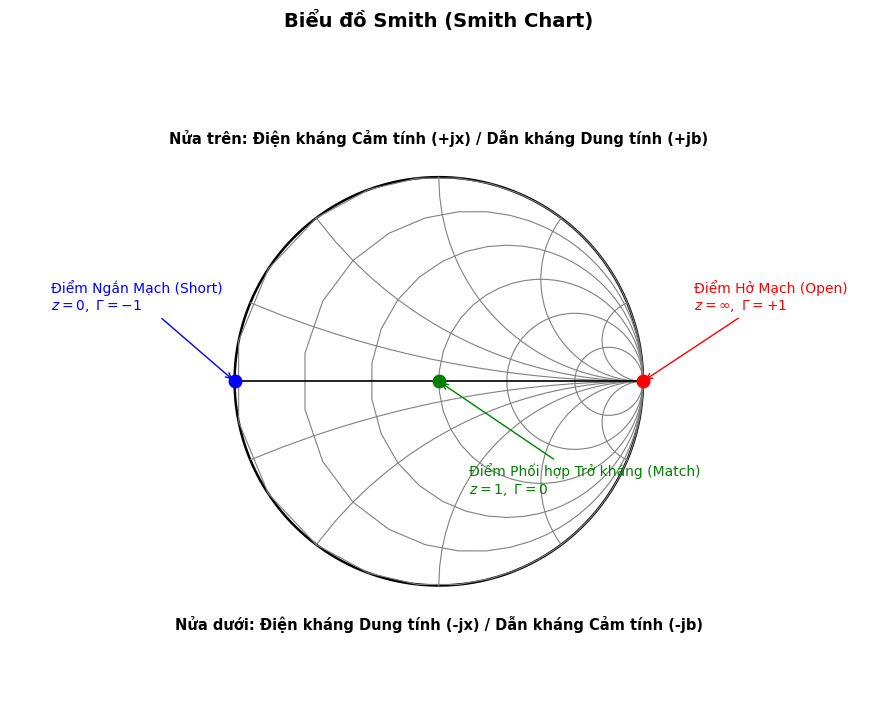
\includegraphics[width=\linewidth,height=5.7cm,keepaspectratio]{01_smith_chart.png}\\[2pt]
      {\scriptsize Tải chuẩn hóa $z_L=0{,}6-j0{,}8$ ($y_L=0{,}6+j0{,}8$) $\to$ tâm $z=1+j0$.}
    \end{column}
    \begin{column}{0.53\textwidth}
      \begin{block}{4 Tiêu chí so sánh kỹ thuật}
        \begin{enumerate}
          \item \textbf{Băng thông ($S_{11}\le-10\dB$):} tương ứng $\mathrm{VSWR}\le 1{,}92$ ($>90\%$ công suất truyền), yêu cầu phủ trọn băng 5G n78 ($3{,}3$--$3{,}7\GHz$).
          \item \textbf{Suy hao chèn ($S_{21}$):} đánh giá tổn hao trên mạch tại $3{,}5\GHz$.
          \item \textbf{Độ nhạy dung sai chế tạo:} khảo sát Parametric Sweep ($\pm5\%$, $\pm10\%$) và Monte Carlo Yield.
          \item \textbf{Kích thước vật lý:} diện tích chiếm dụng trên nền PCB FR-4 ($\varepsilon_r=4{,}4$, $h=1{,}6\,$mm, $t=0{,}035\,$mm, $\tan\delta=0{,}02$).
        \end{enumerate}
      \end{block}
    \end{column}
  \end{columns}
\end{frame}

% =====================================================================
\section{Phương pháp 1: Mạng LC (L-section)}
% =====================================================================

% SLIDE 5
\begin{frame}{PP1 (Mạng LC): Nguyên lý \& Tính toán thiết kế}
  \begin{columns}[c,onlytextwidth]
    \begin{column}{0.53\textwidth}
      \centering
      \adjustbox{max width=\linewidth}{%
        \begin{tikzpicture}[font=\scriptsize,>=Stealth,
          blk/.style={draw,minimum height=1.0cm,align=center,inner sep=3pt}]
          \node[blk,minimum width=1.4cm] (src) at (0,0) {Nguồn\\$Z_0=50\,\Omega$};
          \node[blk,minimum width=1.9cm] (ld) at (6.8,0) {Tải\\$Z_L=30-j40\,\Omega$};
          \draw (src.east) -- (2.8,0);
          \draw[decorate,decoration={coil,aspect=0.5,segment length=3.5pt,amplitude=3pt}] (2.8,0) -- (4.1,0);
          \draw (4.1,0) -- (ld.west);
          \node[above=4pt] at (3.45,0) {$L_s=2{,}933\,$nH};
          \fill (2.0,0) circle (1.5pt);
          \draw (2.0,0) -- (2.0,-0.65);
          \draw (1.7,-0.65) -- (2.3,-0.65);
          \draw (1.7,-0.85) -- (2.3,-0.85);
          \draw (2.0,-0.85) -- (2.0,-1.3);
          \draw (1.65,-1.3) -- (2.35,-1.3);
          \draw (1.82,-1.4) -- (2.18,-1.4);
          \node[right] at (2.3,-0.75) {$C_p=0{,}743\,$pF};
        \end{tikzpicture}}
      \vspace{4pt}
      \begin{block}{Tính toán tại $f_0=3{,}5\GHz$ ($R_L < \Zo$)}
        \small
        \begin{itemize}
          \item $X'=\sqrt{R_L(\Zo-R_L)}=\sqrt{30\cdot20}=24{,}495\,\Omega$
          \item $\omega_0 L_s = X'-X_L = 64{,}495\,\Omega \Rightarrow \mathbf{L_s = 2{,}933\,\mathrm{nH}}$
          \item $\omega_0 C_p = \dfrac{X'}{R_L\Zo} = 0{,}01633\,\mathrm{S} \Rightarrow \mathbf{C_p = 0{,}743\,\mathrm{pF}}$
          \item Phẩm chất thấp $\mathbf{Q = \sqrt{\Zo/R_L-1} = 0{,}816}$ (băng thông rộng).
          \item {\footnotesize Nghiệm 2 dùng 2 cuộn cảm ($0{,}705\,$nH và $2{,}785\,$nH) nên không chọn.}
        \end{itemize}
      \end{block}
    \end{column}
    \begin{column}{0.44\textwidth}
      \centering
      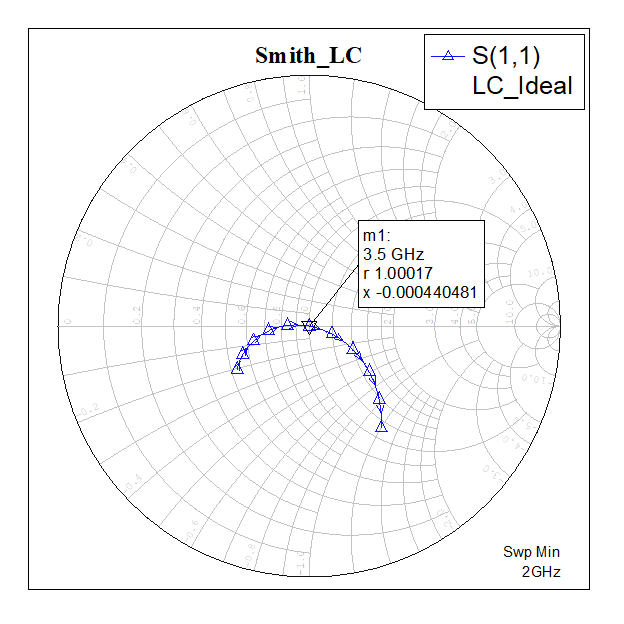
\includegraphics[width=\linewidth,height=6.1cm,keepaspectratio]{02_smith_LC.png}\\[2pt]
      {\scriptsize Biểu đồ Smith đáp ứng $S_{11}$ mạng LC trên AWR.}
    \end{column}
  \end{columns}
\end{frame}

% SLIDE 6
\begin{frame}{PP1 (Mạng LC): Mô phỏng Schematic, Layout \& Tham số S (AWR)}
  \begin{columns}[c,onlytextwidth]
    \begin{column}{0.46\textwidth}
      \centering
      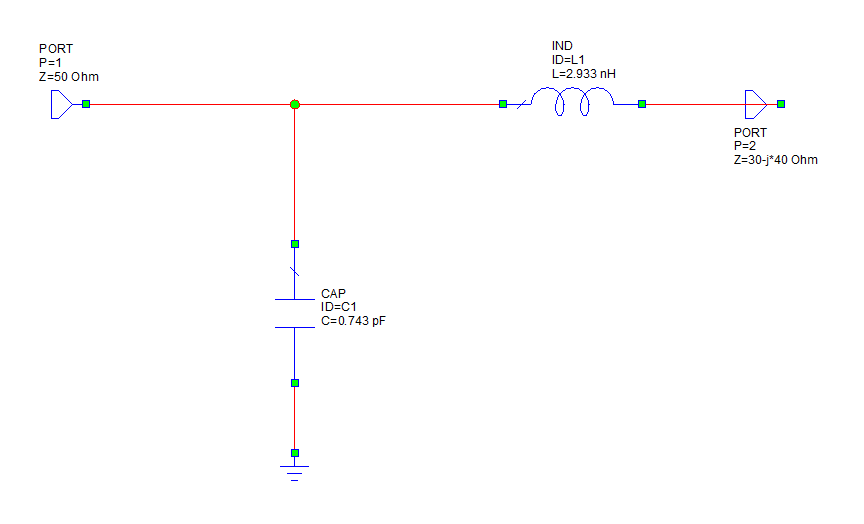
\includegraphics[width=0.49\linewidth,height=2.8cm,keepaspectratio]{05_schematic_LC.png}\hfill
      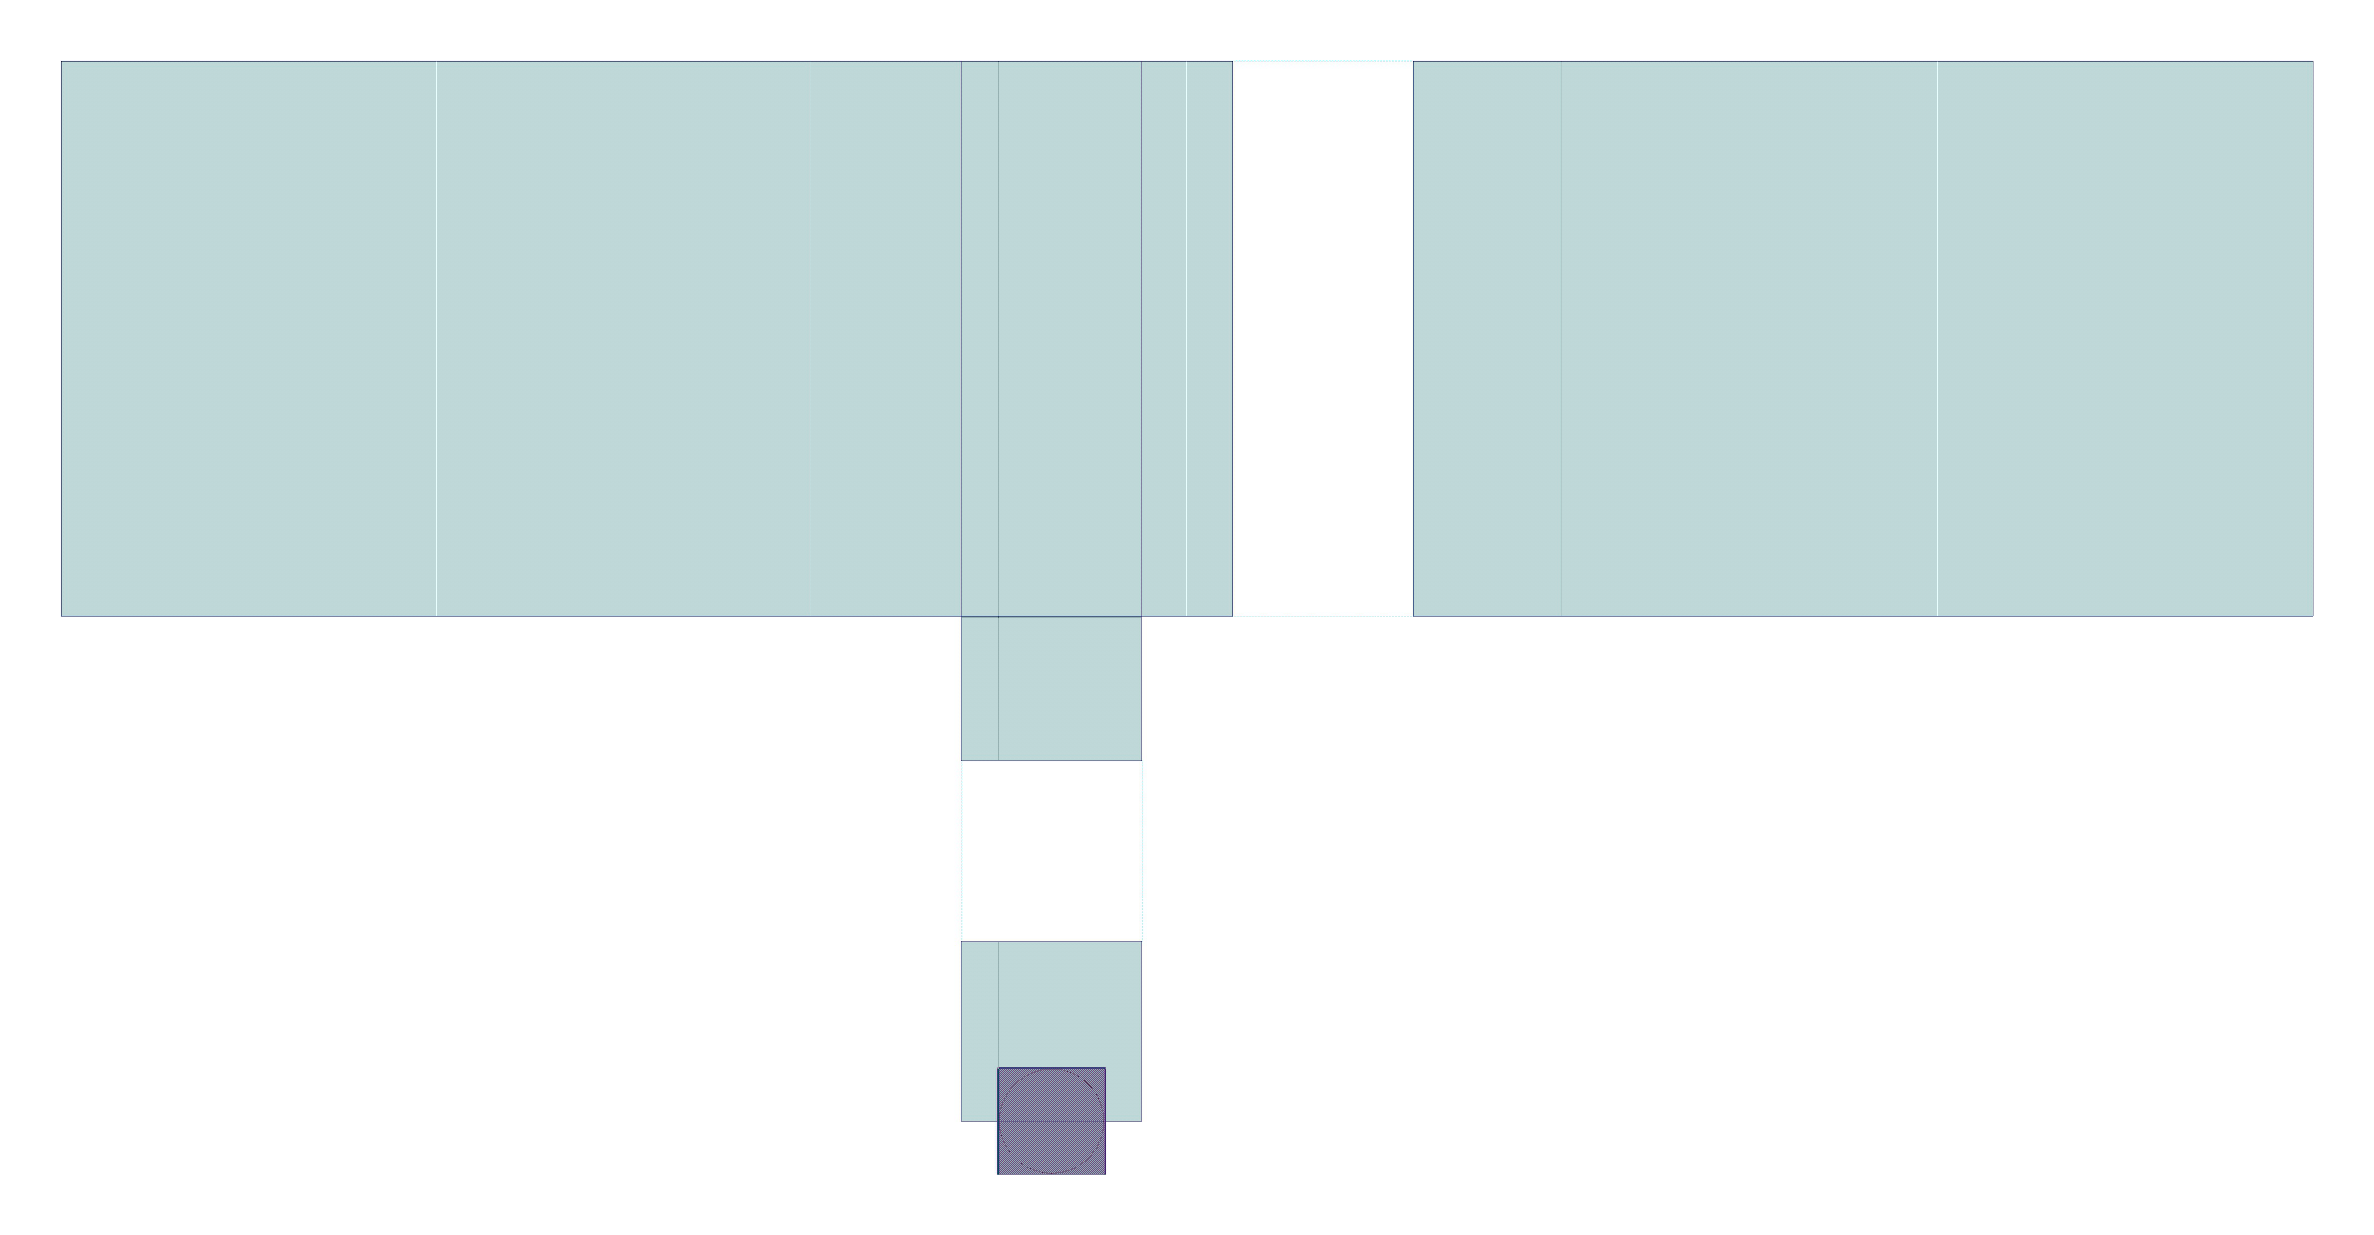
\includegraphics[width=0.49\linewidth,height=2.8cm,keepaspectratio]{05b_layout_LC.png}\\[2pt]
      {\scriptsize Schematic (trái) và Layout FR-4 trên AWR (phải).}\\[4pt]
      \begin{block}{Kết quả mô phỏng (mô hình lý tưởng)}
        \small
        \begin{itemize}
          \item $f_{center} = 3{,}50\GHz$, \quad $\mathbf{S_{11} = -72{,}55\dB}$
          \item $\mathbf{\mathrm{BW}_{-10\dB} = 2323\MHz}$ ($\mathbf{66{,}4\%}$, $2{,}121$--$4{,}444\GHz$)
          \item $S_{21}@3{,}5\GHz = 0{,}00\dB$
        \end{itemize}
      \end{block}
    \end{column}
    \begin{column}{0.51\textwidth}
      \centering
      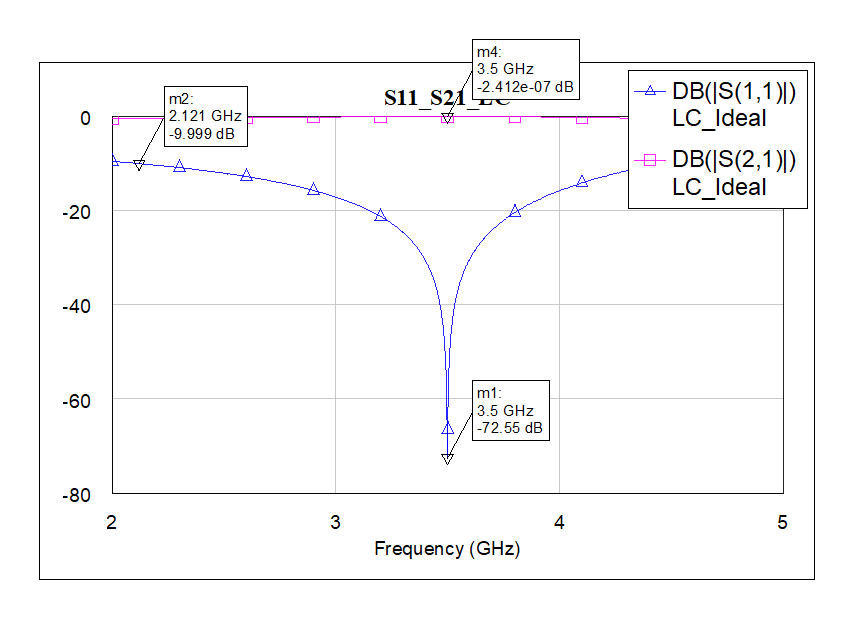
\includegraphics[width=\linewidth,height=6.1cm,keepaspectratio]{06_S11_S21_LC.png}\\[2pt]
      {\scriptsize Đáp ứng $S_{11}$, $S_{21}$ của mạng LC trên AWR ($2$--$5\GHz$).}
    \end{column}
  \end{columns}
\end{frame}

% SLIDE 7
\begin{frame}{PP1 (Mạng LC): Khảo sát dung sai (Parametric Sweep)}
  \begin{columns}[c,onlytextwidth]
    \begin{column}{0.52\textwidth}
      \centering
      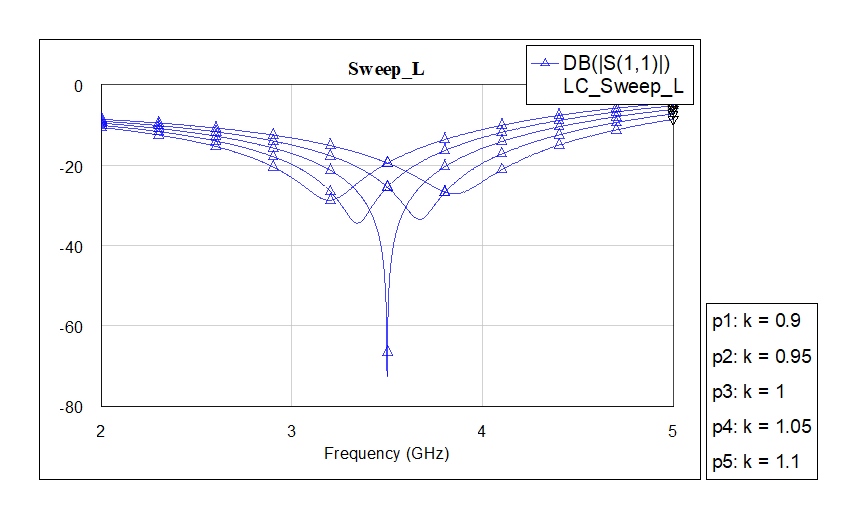
\includegraphics[width=\linewidth,height=2.95cm,keepaspectratio]{07a_sweep_LC_L.png}\\[2pt]
      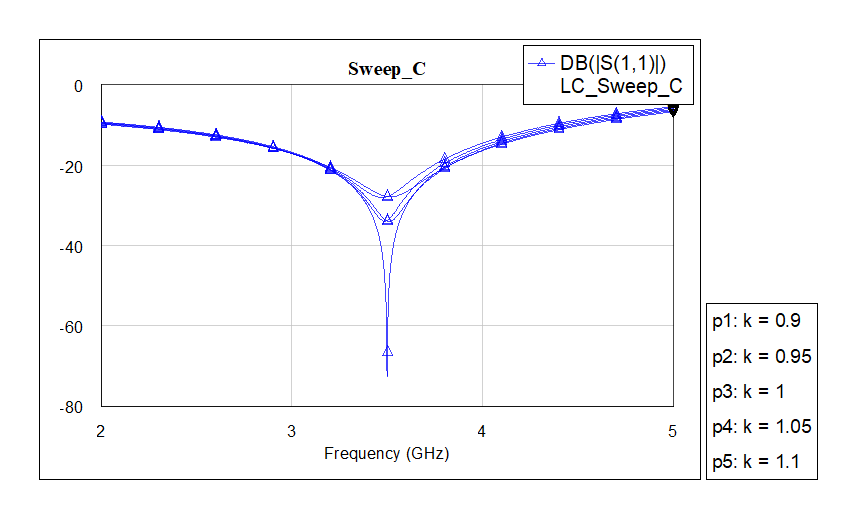
\includegraphics[width=\linewidth,height=2.95cm,keepaspectratio]{07b_sweep_LC_C.png}\\[1pt]
      {\scriptsize Quét riêng lẻ $L_s$ (trên) và $C_p$ (dưới) trên AWR ($\pm5\%$, $\pm10\%$).}
    \end{column}
    \begin{column}{0.45\textwidth}
      \begin{block}{Tóm tắt độ nhạy ($\pm5\%$, $\pm10\%$)}
        \centering\footnotesize
        \begin{tabular}{@{}lccc@{}}
          \toprule
          \textbf{Quét} & \textbf{Sai số} & $\Delta f_{\max}$ & $S_{11}@3{,}5$ \\
          \midrule
          $L_s$ & $\pm5\%$ & $+170\MHz$ & $-25{,}40\dB$ \\
          $L_s$ & $\pm10\%$ & $\mathbf{+350\MHz}$ & $\mathbf{-19{,}42\dB}$ \\
          \midrule
          $C_p$ & $\pm5\%$ & $-15\MHz$ & $-33{,}91\dB$ \\
          $C_p$ & $\pm10\%$ & $-30\MHz$ & $-27{,}88\dB$ \\
          \bottomrule
        \end{tabular}
      \end{block}
      \begin{exampleblock}{Nhận xét}
        \small
        \begin{itemize}
          \item Cuộn cảm $L_s$ ảnh hưởng mạnh hơn tụ $C_p$ rất nhiều.
          \item Mọi kịch bản đều giữ $S_{11}\le-19{,}4\dB$ tại $3{,}5\GHz$.
        \end{itemize}
      \end{exampleblock}
    \end{column}
  \end{columns}
\end{frame}

% =====================================================================
\section{Phương pháp 2: Single-Stub hở mạch}
% =====================================================================

% SLIDE 8
\begin{frame}{PP2 (Single-Stub): Nguyên lý \& Tính toán thiết kế}
  \begin{columns}[c,onlytextwidth]
    \begin{column}{0.55\textwidth}
      \centering
      \adjustbox{max width=\linewidth}{%
        \begin{tikzpicture}[font=\scriptsize,>=Stealth,
          blk/.style={draw,minimum height=0.95cm,align=center,inner sep=3pt}]
          \node[blk,minimum width=1.3cm] (src) at (0,0) {Nguồn\\$Z_0$};
          \node[blk,minimum width=1.6cm] (ld) at (7.0,0) {Tải\\$Z_L\,(y_L)$};
          \draw[thick] (src.east) -- (ld.west);
          \draw[thick] (4.2,0) -- (4.2,1.5);
          \fill[white,draw] (4.2,1.58) circle (2pt);
          \node[right] at (4.3,1.1) {Stub hở mạch};
          \draw[<->] (3.6,0.08) -- (3.6,1.5) node[midway,left] {$l$};
          \draw[dashed] (4.2,0) -- (4.2,-0.65);
          \draw[dashed] (6.2,0) -- (6.2,-0.65);
          \draw[<->] (4.2,-0.5) -- (6.2,-0.5) node[midway,below] {$d$};
          \node[above] at (2.1,0.05) {$y_{in}=1$};
          \node[above] at (5.2,0.05) {$y(d)=1+jb$};
        \end{tikzpicture}}
      \vspace{2pt}
      \begin{block}{Tính toán trên FR-4 ($\varepsilon_r=4{,}4$, $h=1{,}6\,$mm)}
        \footnotesize
        $W=3{,}083\,$mm, $\varepsilon_{eff}=3{,}3323$, $\lambda_g=46{,}922\,$mm. Giải $t^2-4t+1=0$:
        \vspace{2pt}
        \centering
        \adjustbox{max width=\linewidth}{%
        \begin{tabular}{@{}ccccc@{}}
          \toprule
          \textbf{Nghiệm} & $d$ (mm) & $y(d)$ & $l$ hở (mm) & $d+l$ \\
          \midrule
          1 & $1{,}955$ ($0{,}0417\lambda_g$) & $1+j1{,}155$ & $17{,}06$ ($0{,}3636\lambda_g$) & $19{,}0\,$mm \\
          2 & $9{,}775$ ($0{,}2083\lambda_g$) & $1-j1{,}155$ & $6{,}40$ ($0{,}1364\lambda_g$) & $16{,}2\,$mm \\
          \bottomrule
        \end{tabular}}
      \end{block}
    \end{column}
    \begin{column}{0.42\textwidth}
      \centering
      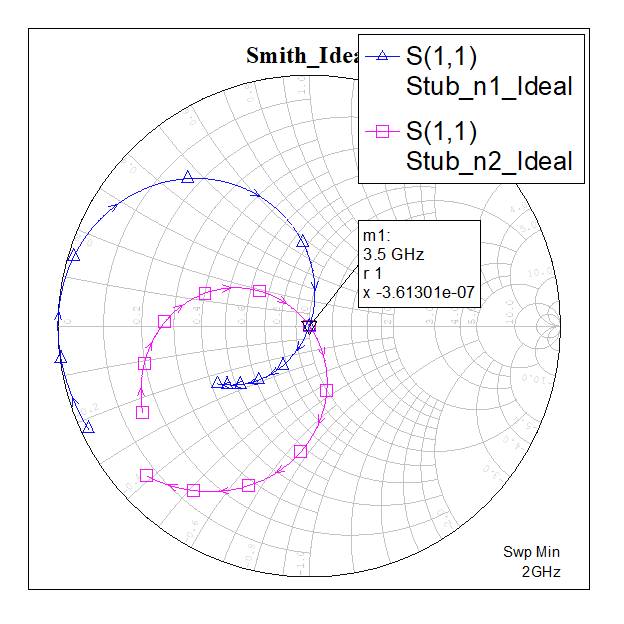
\includegraphics[width=\linewidth,height=6.1cm,keepaspectratio]{03_smith_stub.png}\\[2pt]
      {\scriptsize Biểu đồ Smith hai bộ nghiệm trên AWR.}
    \end{column}
  \end{columns}
\end{frame}

% SLIDE 9
\begin{frame}{PP2 (Single-Stub): Layout, Mô phỏng AWR \& Tinh chỉnh}
  \begin{columns}[T,onlytextwidth]
    \begin{column}{0.49\textwidth}
      \centering
      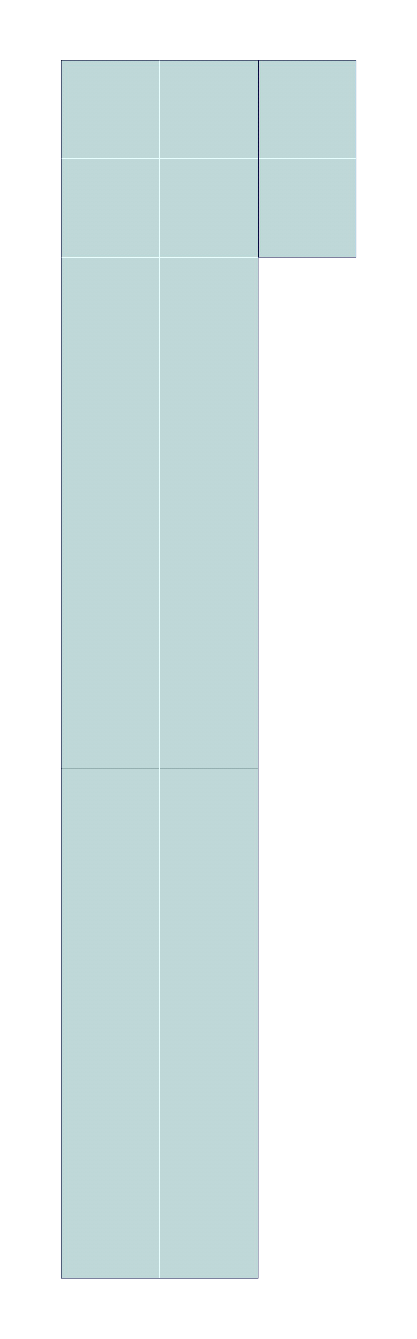
\includegraphics[width=0.25\linewidth,height=3.55cm,keepaspectratio]{09b_layout_stub1.png}\hfill
      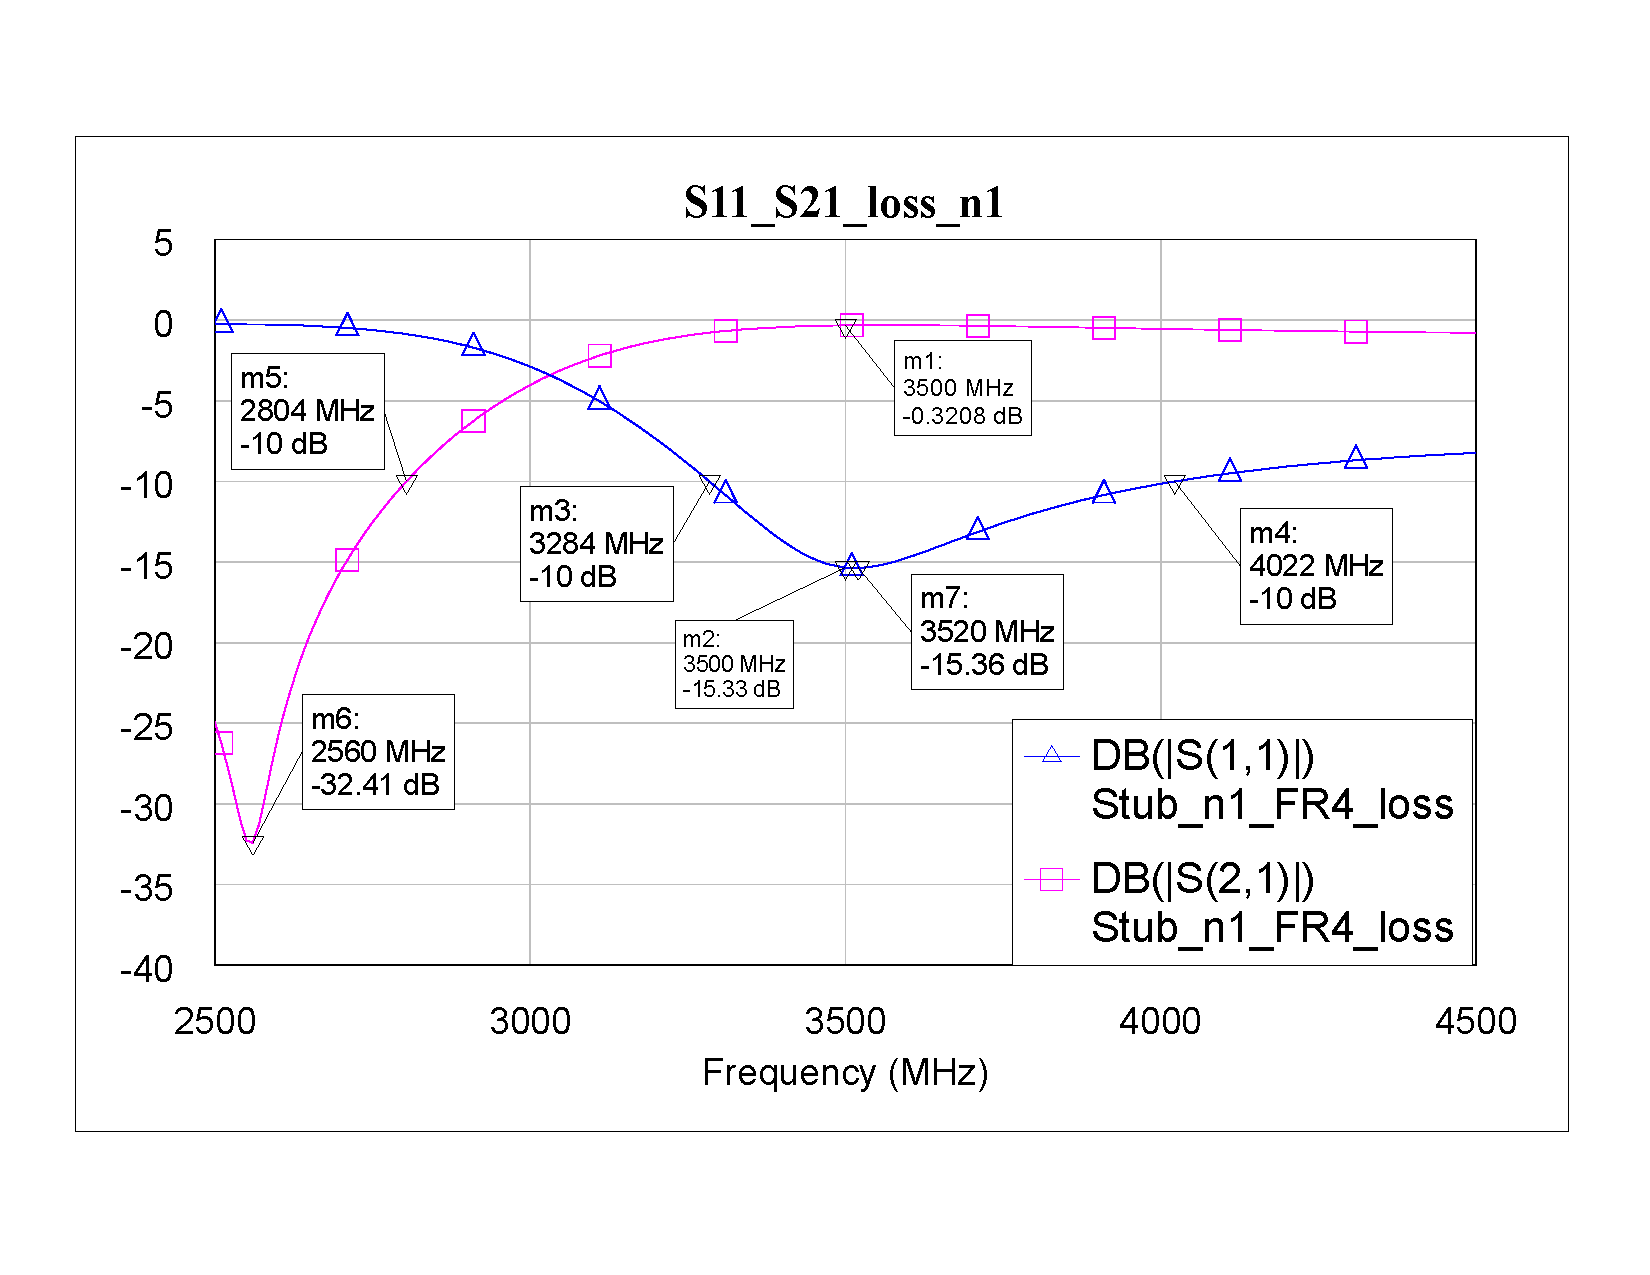
\includegraphics[width=0.73\linewidth,height=3.55cm,keepaspectratio]{10_S11_S21_stub1.pdf}\\[2pt]
      {\scriptsize Nghiệm 1: Layout AWR \& $S_{11}, S_{21}$ ($d=1{,}50\,$mm, $l=15{,}75\,$mm)}
    \end{column}
    \begin{column}{0.49\textwidth}
      \centering
      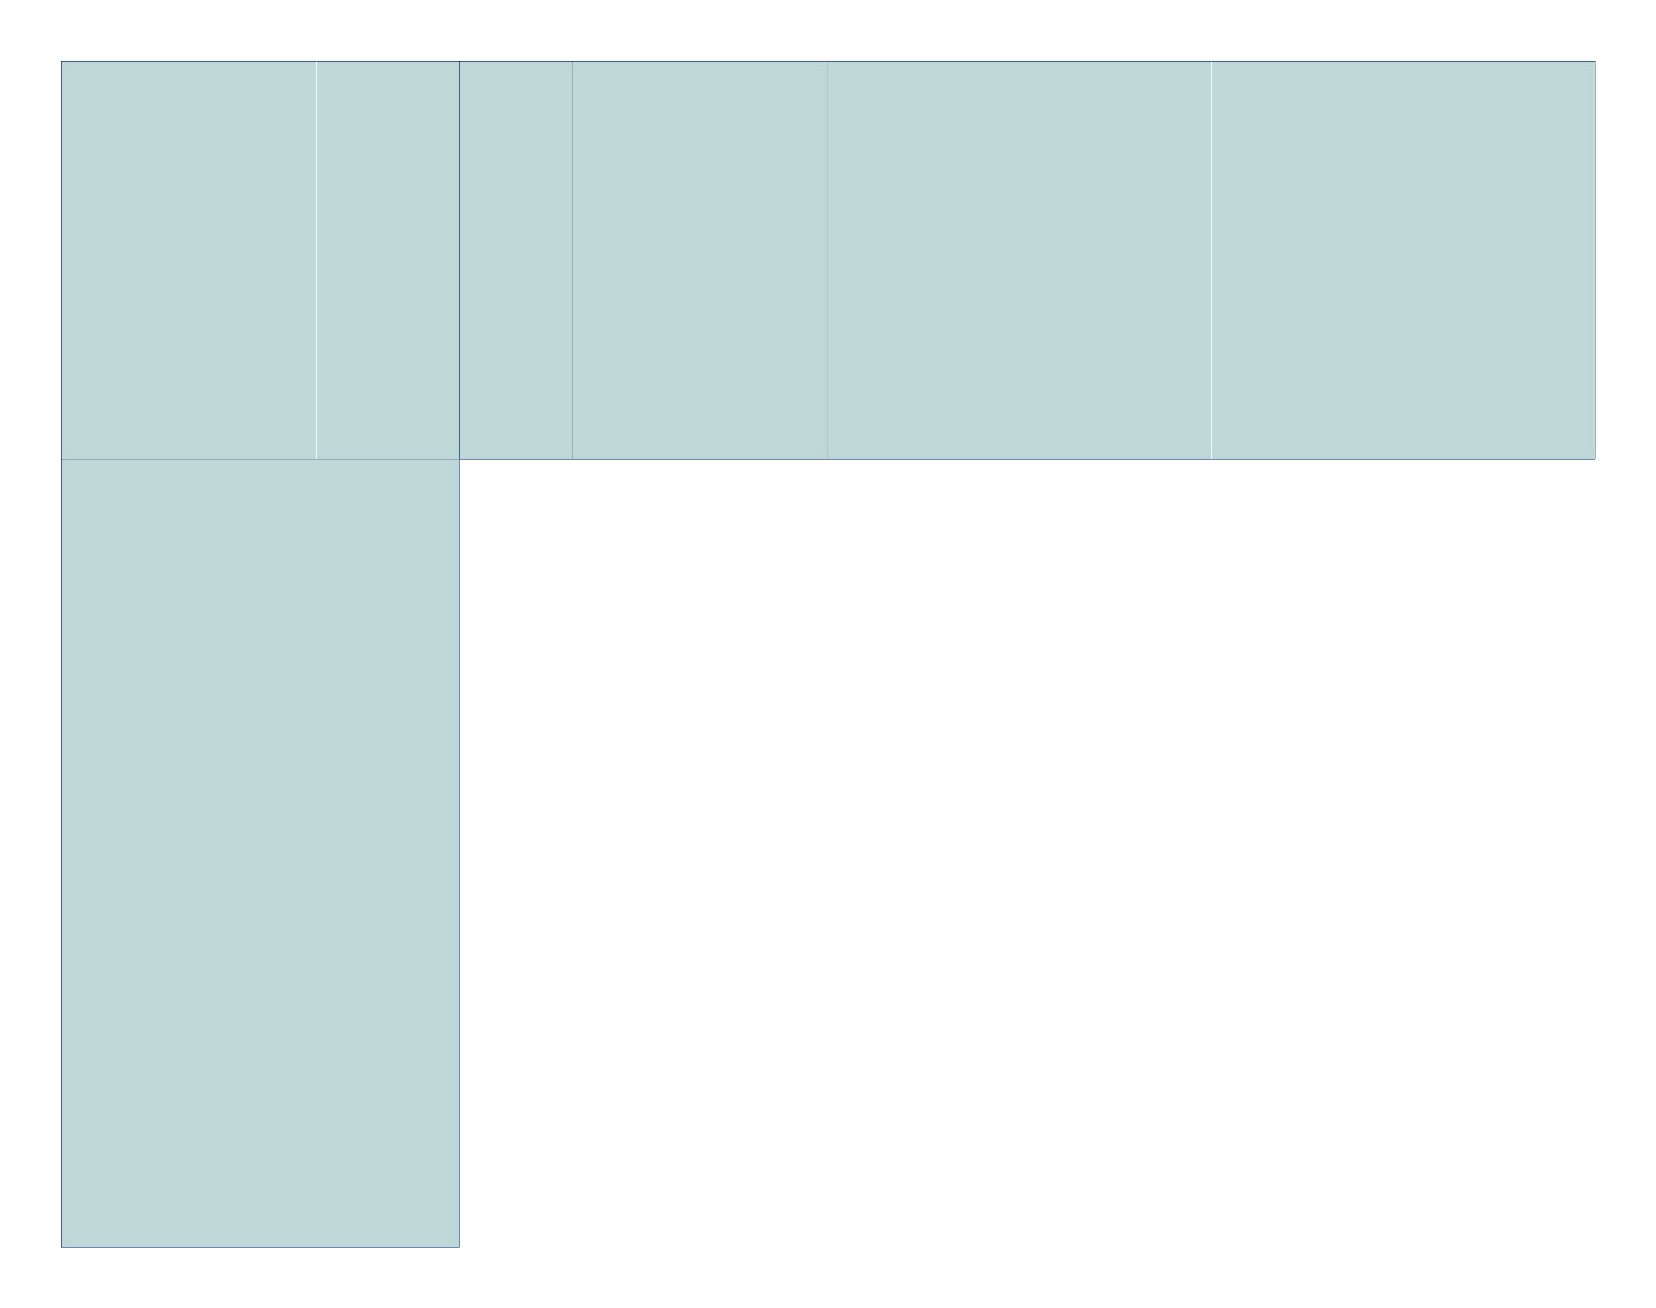
\includegraphics[width=0.35\linewidth,height=3.55cm,keepaspectratio]{09c_layout_stub2.png}\hfill
      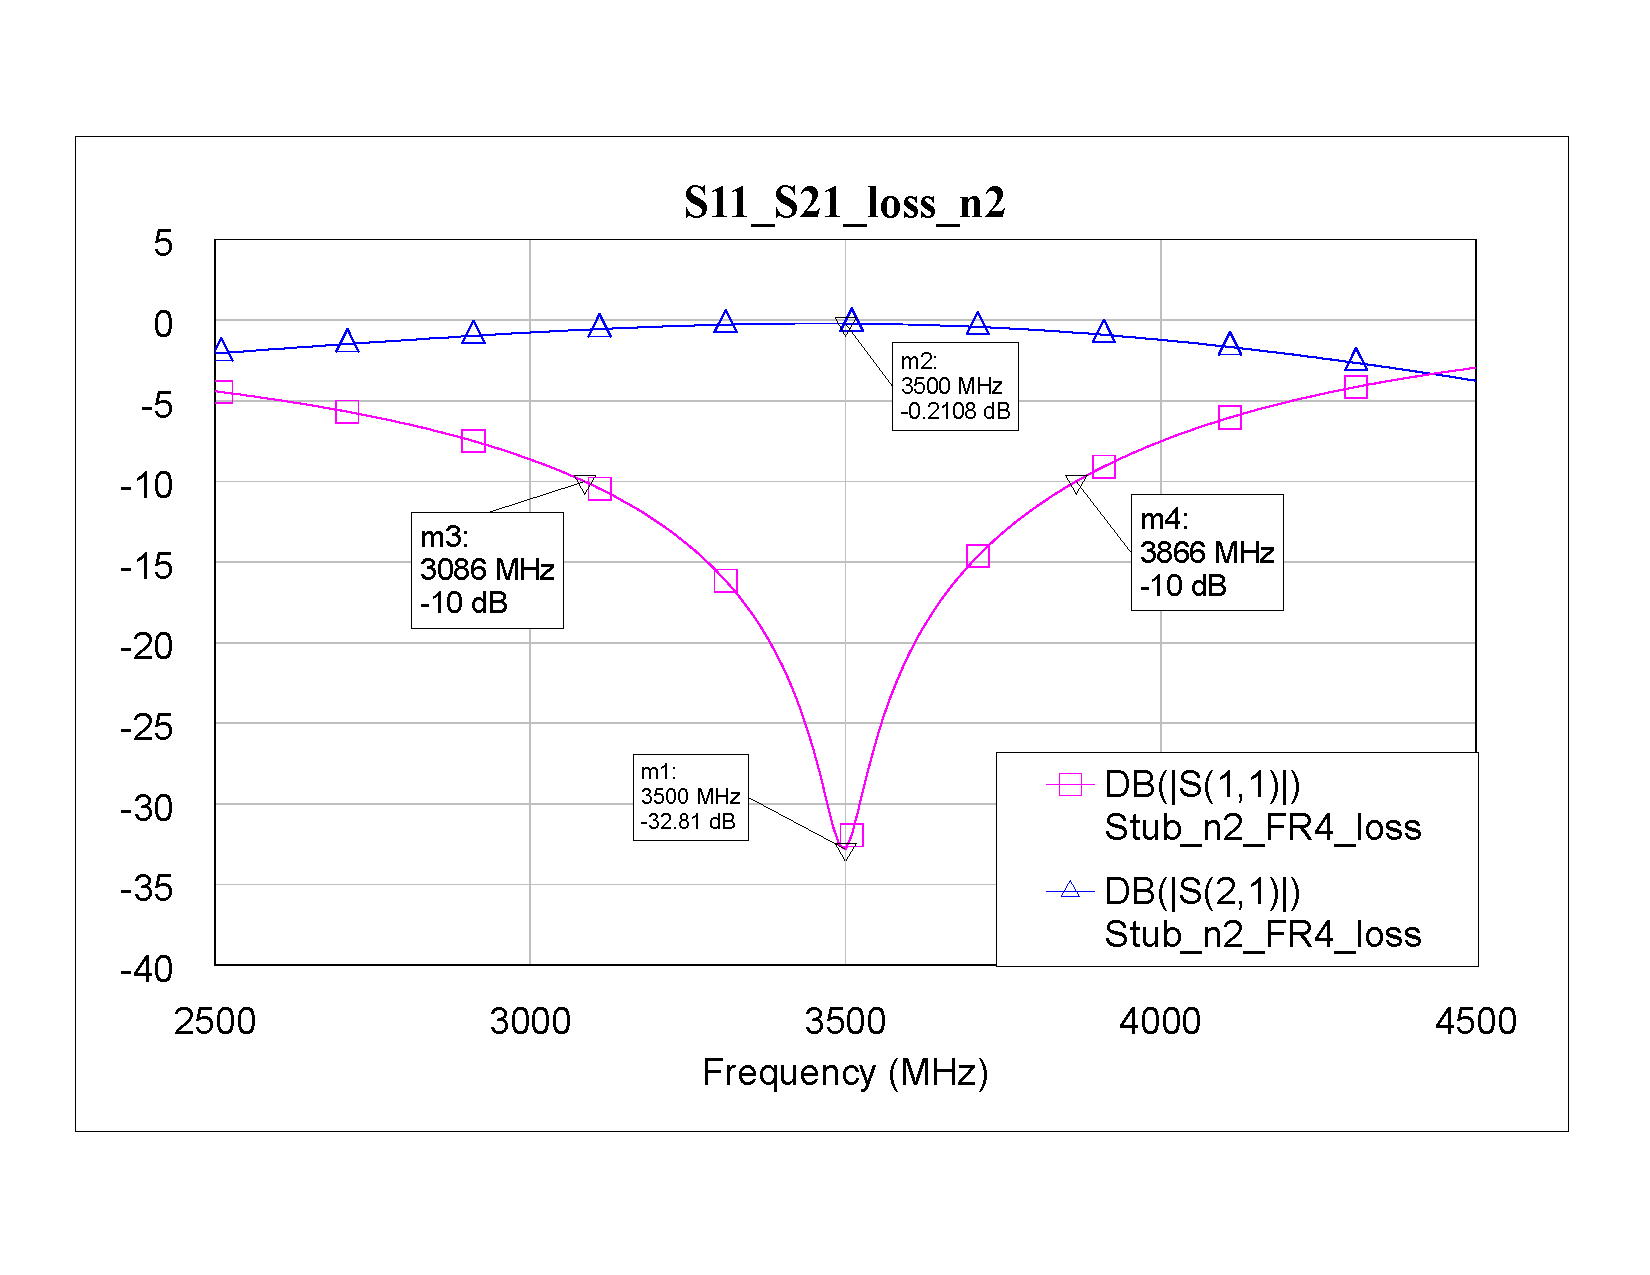
\includegraphics[width=0.63\linewidth,height=3.55cm,keepaspectratio]{11_S11_S21_stub2.pdf}\\[2pt]
      {\scriptsize Nghiệm 2: Layout AWR \& $S_{11}, S_{21}$ ($d=8{,}65\,$mm, $l=6{,}00\,$mm)}
    \end{column}
  \end{columns}
  \vspace{4pt}
  \centering
  \adjustbox{max width=\linewidth}{%
  \footnotesize
  \begin{tabular}{@{}lcccccc@{}}
    \toprule
    \textbf{Phương án} ($\tan\delta=0{,}02$, $W=3{,}034\,$mm) & $f_{min}$ & $S_{11}@3{,}5$ & $\mathrm{BW}_{-10\dB}$ & $S_{21}@3{,}5$ & $d+l$ & Diện tích đồng \\
    \midrule
    Nghiệm 1 ($l$ giảm $7{,}7\%$, $d$ giảm $23{,}3\%$) & $3{,}52\GHz$ & $-15{,}33\dB$ & $738\MHz$ ($21{,}1\%$) & $-0{,}321\dB$ & $17{,}25\,$mm & $\approx52{,}3\,\mathrm{mm}^2$ \\
    \textbf{Nghiệm 2} ($l$ giảm $6{,}3\%$, $d$ giảm $11{,}5\%$) & $\mathbf{3{,}50\GHz}$ & $\mathbf{-32{,}81\dB}$ & $\mathbf{780\MHz}$ ($\mathbf{22{,}3\%}$) & $\mathbf{-0{,}211\dB}$ & $\mathbf{14{,}65}\,\text{mm}$ & $\mathbf{\approx44{,}4\,\mathrm{mm}^2}$ \\
    \bottomrule
  \end{tabular}}
\end{frame}

% SLIDE 10
\begin{frame}{PP2 (Single-Stub): Khảo sát dung sai (Parametric Sweep)}
  \begin{columns}[T,onlytextwidth]
    \begin{column}{0.49\textwidth}
      \centering
      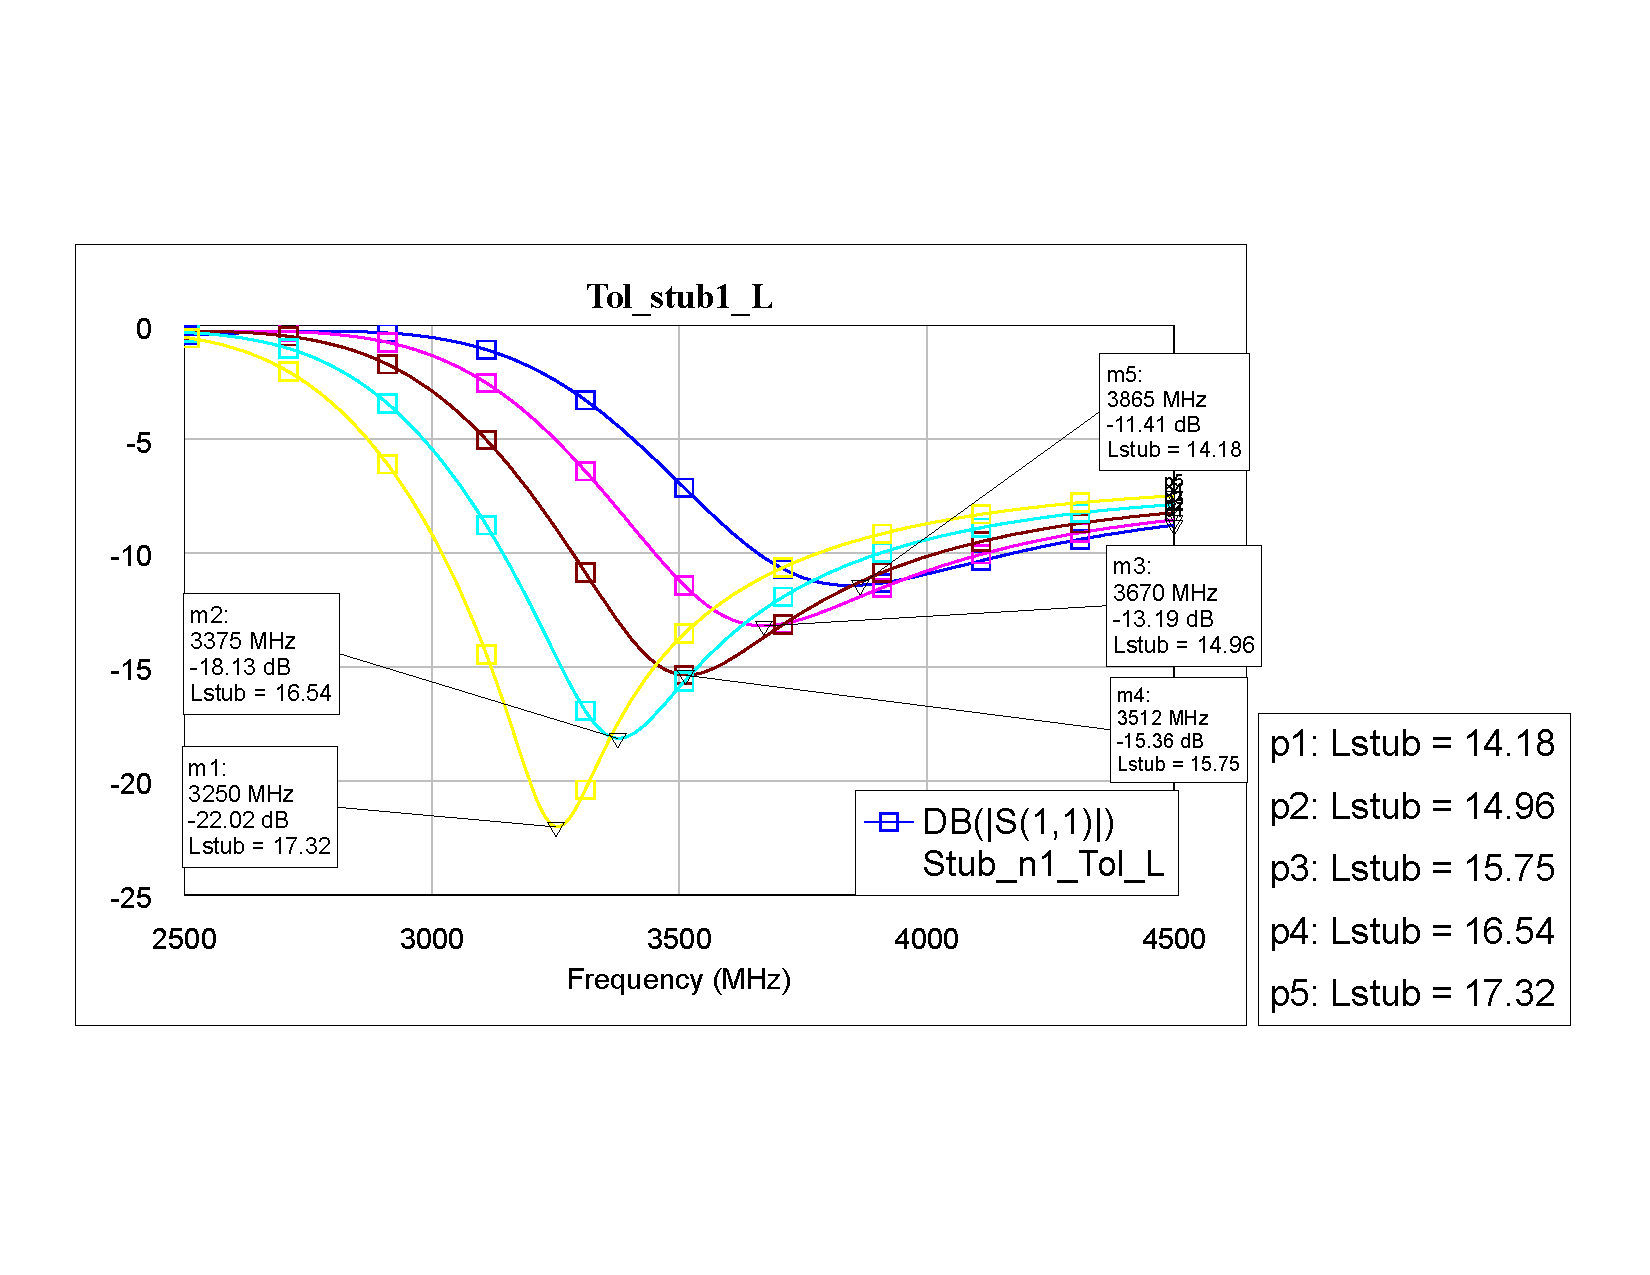
\includegraphics[width=\linewidth,height=4.0cm,keepaspectratio]{16_Tol_stub1_L.pdf}\\[2pt]
      {\scriptsize Nghiệm 1: quét chiều dài stub $l$ ($\pm5\%$, $\pm10\%$)}
    \end{column}
    \begin{column}{0.49\textwidth}
      \centering
      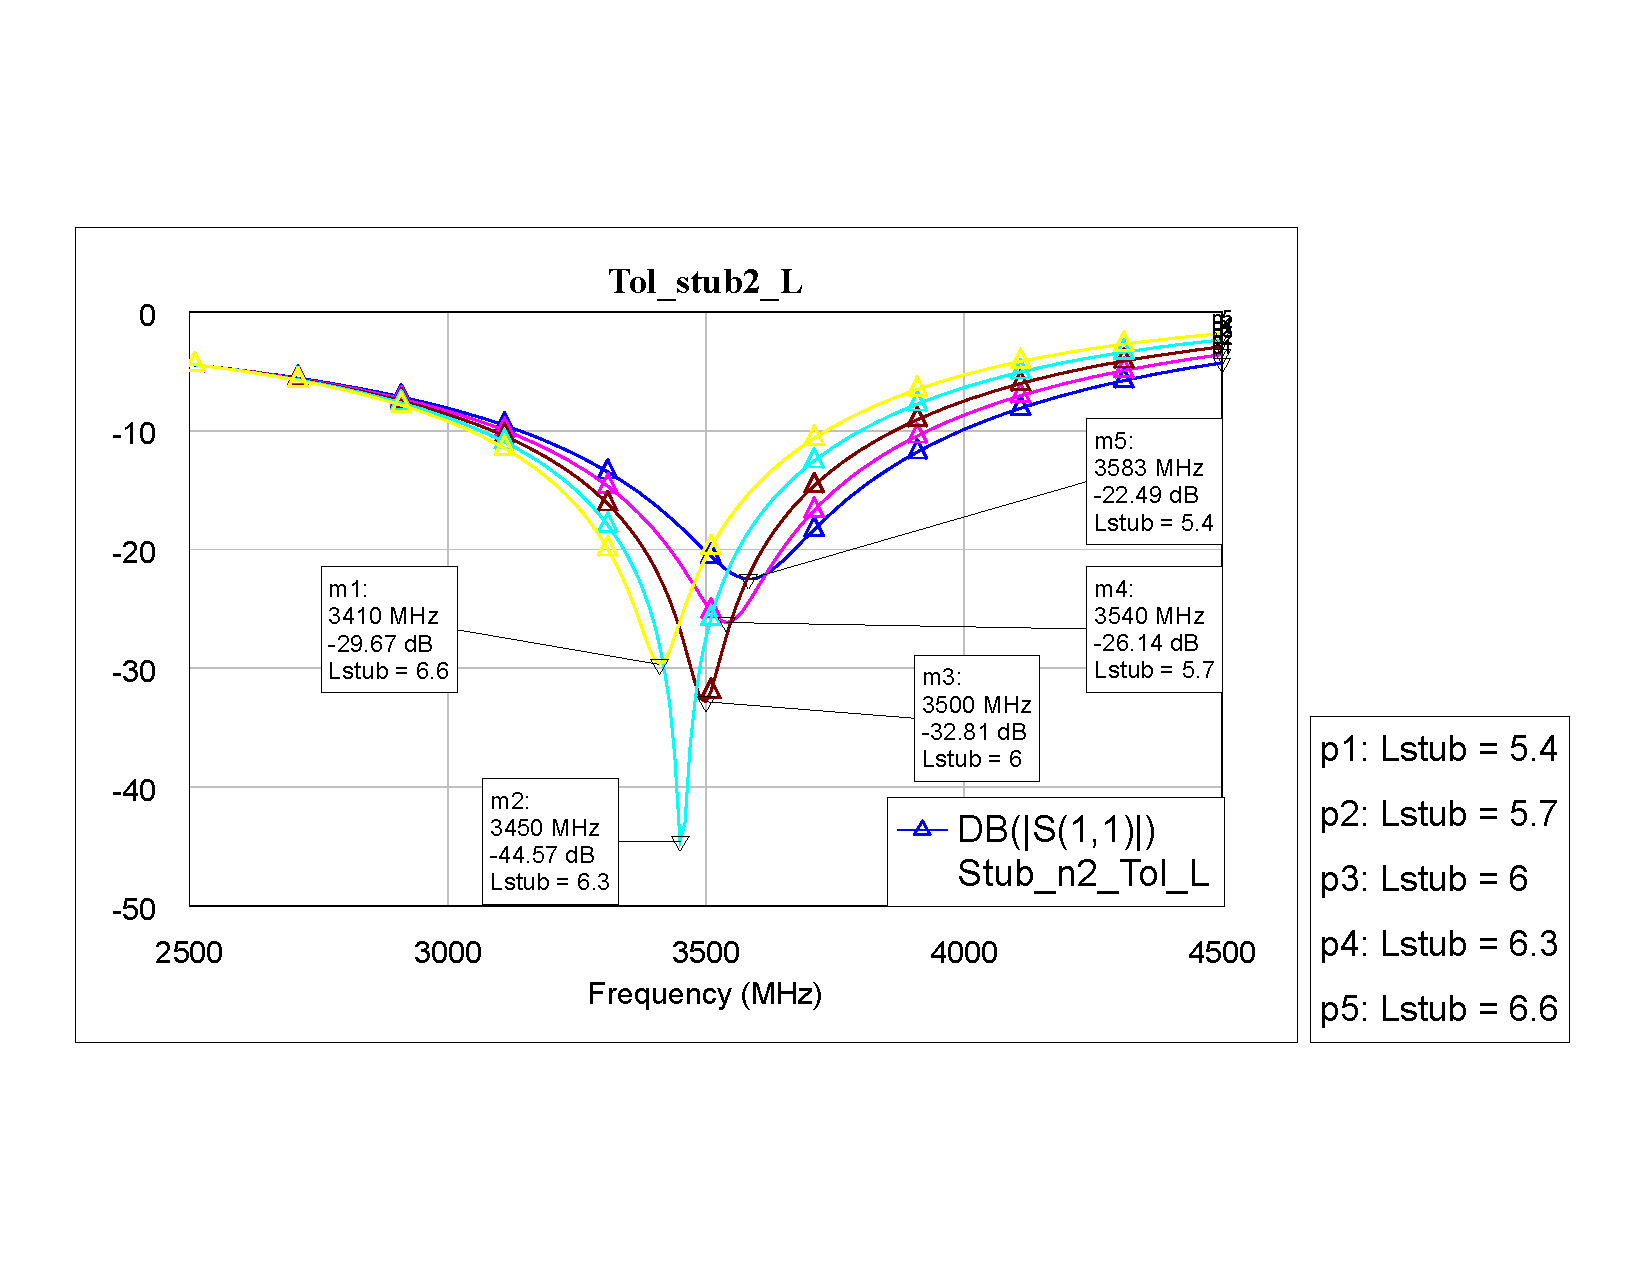
\includegraphics[width=\linewidth,height=4.0cm,keepaspectratio]{18_Tol_stub2_L.pdf}\\[2pt]
      {\scriptsize Nghiệm 2: quét chiều dài stub $l$ ($\pm5\%$, $\pm10\%$)}
    \end{column}
  \end{columns}
  \vspace{4pt}
  \begin{block}{Nhận xét độ nhạy}
    \small
    \begin{itemize}
      \item \textbf{Chiều dài stub $l$ nhạy nhất:} khi lệch $\pm10\%$, Nghiệm 1 dịch từ $3250$--$3865\MHz$ ($-262/+353\MHz$; mức $+10\%$ rơi khỏi băng n78), còn Nghiệm 2 chỉ dịch $\mathbf{-90/+83\MHz}$ ($3410$--$3583\MHz$).
      \item \textbf{Chiều rộng $W$ ít ảnh hưởng:} dịch $<10\MHz$ (N1) và $\pm58\MHz$ (N2, $S_{11}<-29\dB$) $\Rightarrow$ \textbf{chọn Nghiệm 2}.
    \end{itemize}
  \end{block}
\end{frame}

% =====================================================================
\section{Phương pháp 3: Biến áp \texorpdfstring{$\lambda/4$}{lambda/4} kết hợp dây đệm}
% =====================================================================

% SLIDE 11
\begin{frame}{PP3 (Biến áp $\lambda/4$): Nguyên lý \& Tính toán thiết kế}
  \begin{columns}[c,onlytextwidth]
    \begin{column}{0.56\textwidth}
      \centering
      \adjustbox{max width=\linewidth}{%
        \begin{tikzpicture}[font=\scriptsize,>=Stealth,
          blk/.style={draw,minimum height=0.95cm,align=center,inner sep=3pt}]
          \node[blk,minimum width=1.4cm] (src) at (0,0) {Nguồn\\$50\,\Omega$};
          \node[blk,minimum width=2.4cm] (tf) at (2.8,0) {Biến áp $\lambda/4$\\$Z_t=28{,}87\,\Omega$};
          \node[blk,minimum width=1.9cm] (bf) at (5.8,0) {Dây đệm\\$50\,\Omega,\ d_0$};
          \node[blk,minimum width=1.3cm] (ld) at (8.1,0) {Tải\\$Z_L$};
          \draw (src.east) -- (tf.west);
          \draw (tf.east) -- (bf.west);
          \draw (bf.east) -- (ld.west);
          \node[below=2pt] at ($(tf.east)!0.5!(bf.west)$) {$R'_{in}=16{,}67\,\Omega$};
        \end{tikzpicture}}
      \vspace{4pt}
      \begin{block}{Tính toán 2 bước (chọn nghiệm ngắn $V_{min}$)}
        \footnotesize
        \begin{itemize}
          \item \textbf{Dây đệm $50\,\Omega$:} quay $90^\circ$ về $V_{min}$ $\Rightarrow d_0 = \lambda_g/8 = \mathbf{5{,}865}\,\text{mm}$ ($W=3{,}083\,$mm), thu tải thuần thực $R'_{in} = \Zo\dfrac{1-|\GL|}{1+|\GL|} = \mathbf{16{,}667\,\Omega}$.
          \item \textbf{Biến áp $\lambda/4$:} $\mathbf{Z_t = \sqrt{\Zo R'_{in}} = 28{,}868\,\Omega}$ $\Rightarrow$ trên FR-4: $W_t = \mathbf{6{,}947}\,\text{mm}$, $\varepsilon_{eff}=3{,}5763$, $L_t = \lambda_g/4 = \mathbf{11{,}323}\,\text{mm}$.
          \item Tổng chiều dài lý thuyết: $d_0+L_t = 17{,}188\,$mm.
        \end{itemize}
      \end{block}
    \end{column}
    \begin{column}{0.41\textwidth}
      \centering
      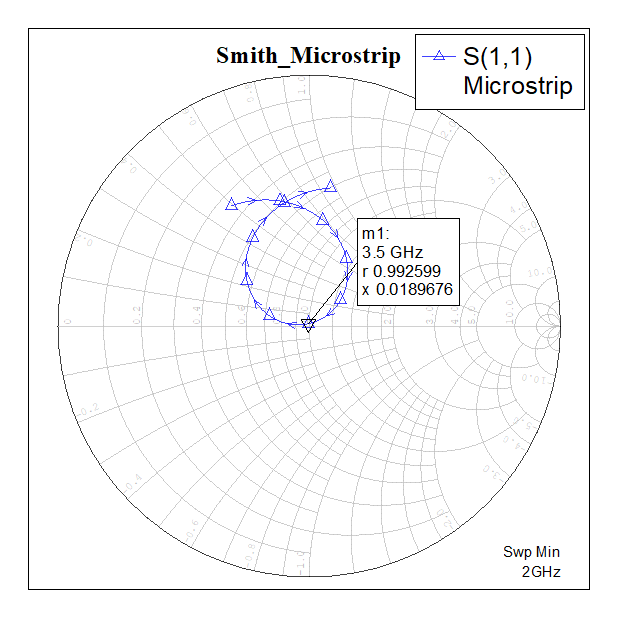
\includegraphics[width=\linewidth,height=6.1cm,keepaspectratio]{04_smith_trans.png}\\[2pt]
      {\scriptsize Quỹ đạo $DP_1 \to TP_2 \to TP_3$ trên Smith.}
    \end{column}
  \end{columns}
\end{frame}

% SLIDE 12
\begin{frame}{PP3 (Biến áp $\lambda/4$): Mô phỏng AWR, Layout \& Hiệu chỉnh}
  \begin{columns}[T,onlytextwidth]
    \begin{column}{0.50\textwidth}
      \centering
      
\includegraphics[width=\linewidth,height=1.85cm,keepaspectratio]{22_layout_vidai.pdf}\\[1pt]
      {\scriptsize Layout FR-4: dài $16{,}385\,$mm, rộng $6{,}947\,$mm, đồng $\approx91{,}2\,\mathrm{mm}^2$.}
      \vspace{2pt}
      \begin{block}{So sánh trước và sau hiệu chỉnh}
        \centering
        \adjustbox{max width=\linewidth}{%
        \scriptsize
        \begin{tabular}{@{}lccc@{}}
          \toprule
          \textbf{Chỉ tiêu} & \textbf{Lý tưởng} & \textbf{Trước tune} & \textbf{Sau tune} \\
          \midrule
          $L_t$ (mm) & $\lambda_g/4$ & $11{,}323$ & $\mathbf{10{,}520}$ ($-7{,}1\%$) \\
          $f_{min}$ (GHz) & $3{,}50$ & $3{,}39$ & $\mathbf{3{,}50}$ \\
          $S_{11}$ đáy (dB) & $-126{,}6$ & $-39{,}96$ & $\mathbf{-39{,}81}$ \\
          $\mathrm{BW}_{-10\dB}$ & $1232\MHz$ & $1204\MHz$ & $\mathbf{1242\MHz}$ ($35{,}5\%$) \\
          \bottomrule
        \end{tabular}}
      \end{block}
      {\scriptsize Lệch $-110\MHz$ do tán sắc FR-4 \& MSTEP; $S_{21}=-0{,}261\dB$.}
    \end{column}
    \begin{column}{0.48\textwidth}
      \centering
      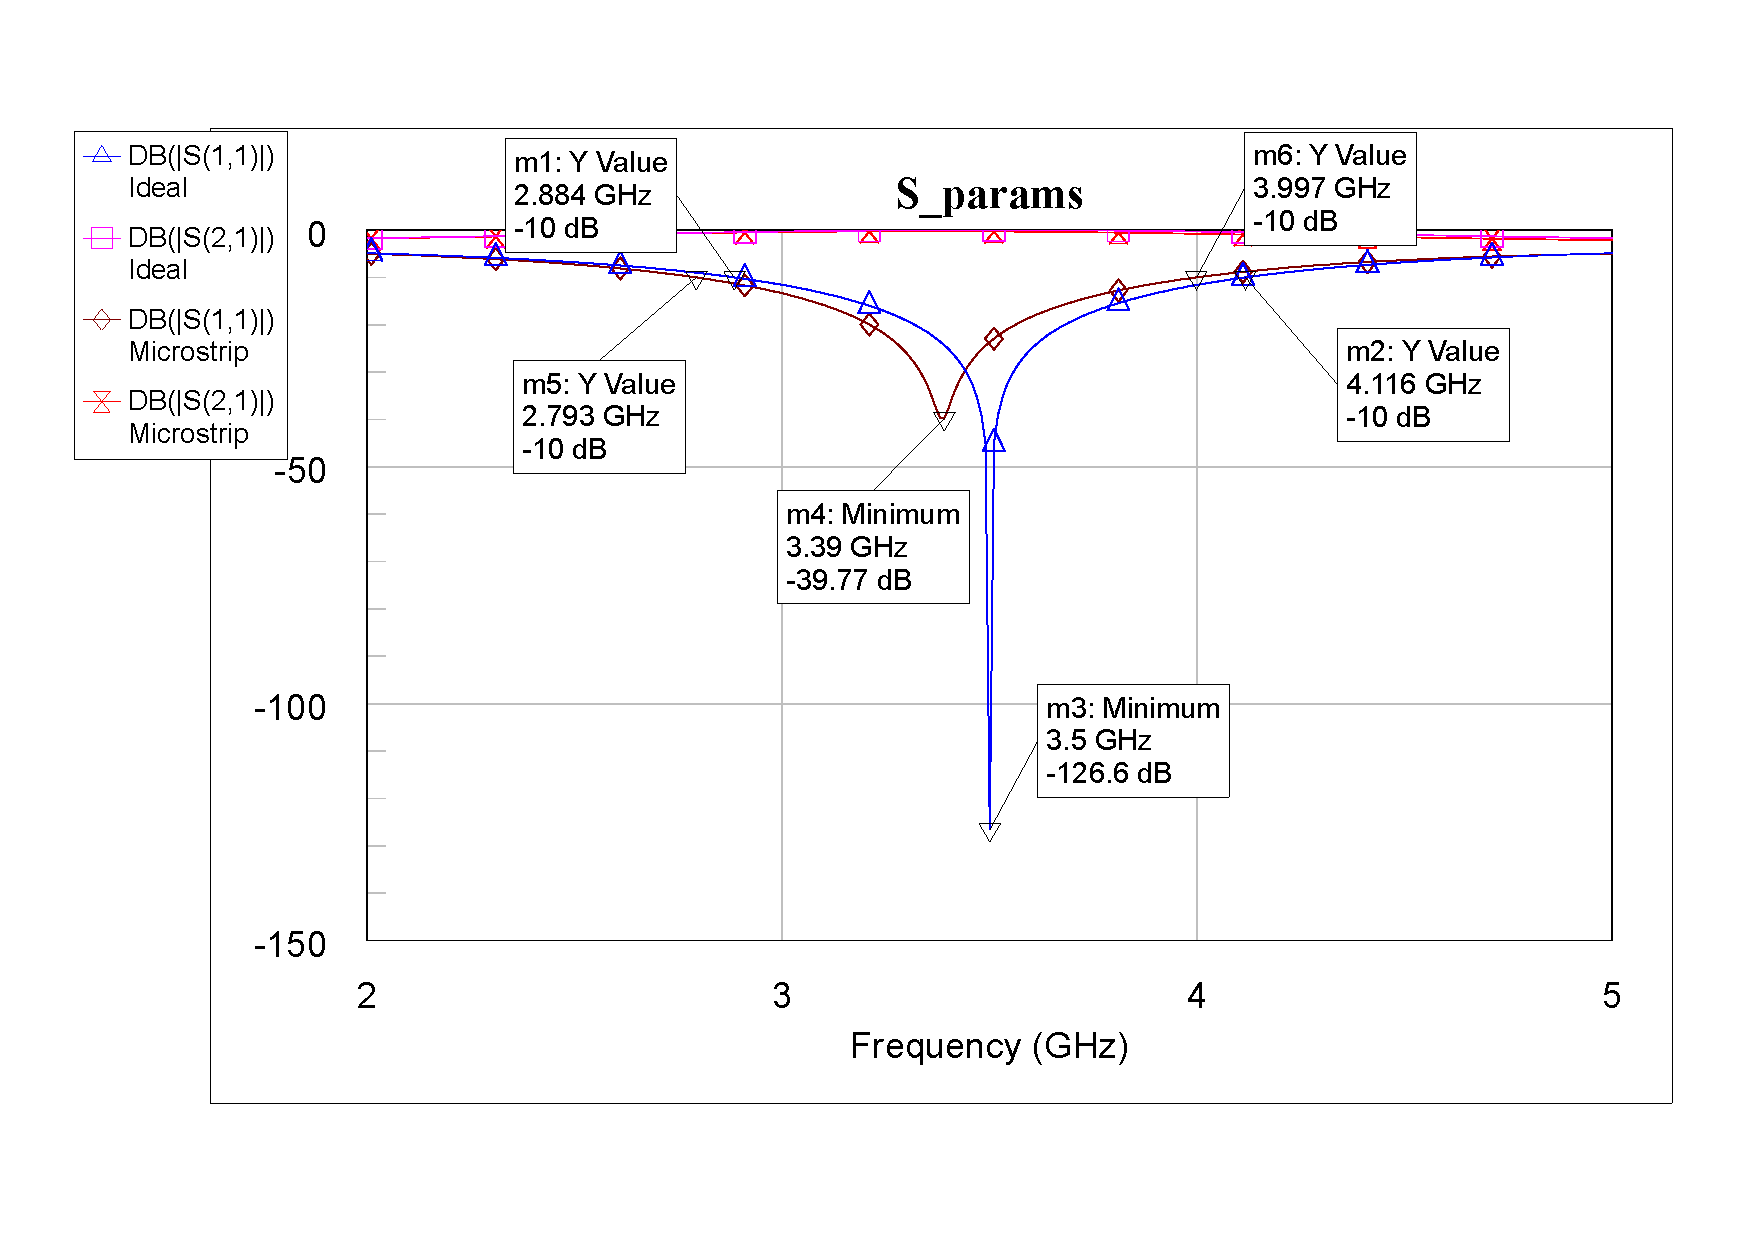
\includegraphics[width=\linewidth,height=2.85cm,keepaspectratio]{25_S11S21_truoc_tune.pdf}\\[2pt]
      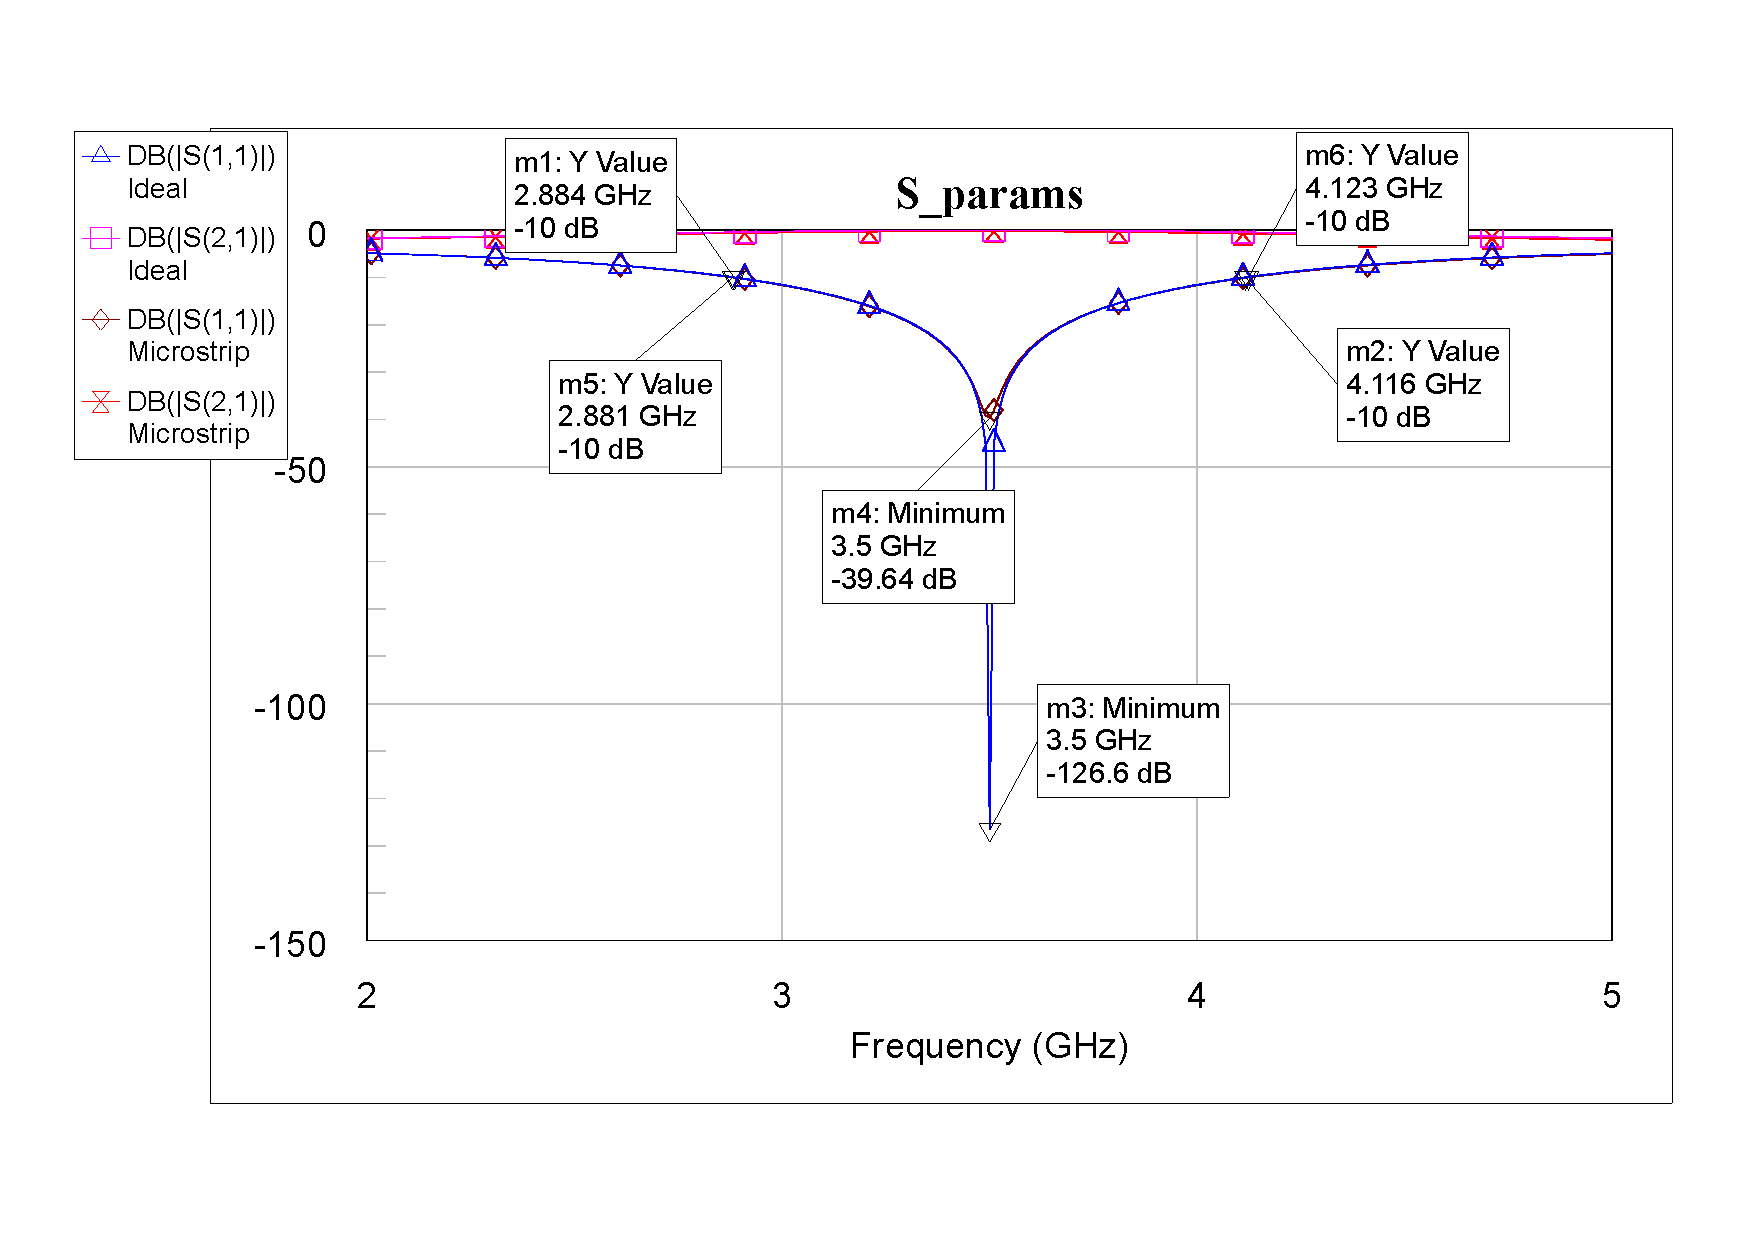
\includegraphics[width=\linewidth,height=2.85cm,keepaspectratio]{26_S11S21_sau_tune.pdf}\\[1pt]
      {\scriptsize $S_{11}, S_{21}$ trước tune (trên) và sau tune $L_t=10{,}52\,$mm (dưới).}
    \end{column}
  \end{columns}
\end{frame}

% SLIDE 13
\begin{frame}{PP3 (Biến áp $\lambda/4$): Khảo sát dung sai \& Monte Carlo Yield}
  \begin{columns}[c,onlytextwidth]
    \begin{column}{0.53\textwidth}
      \begin{block}{Độ nhạy của 5 tham số (Parametric Sweep)}
        \centering
        \adjustbox{max width=\linewidth}{%
        \scriptsize
        \begin{tabular}{@{}lcccc@{}}
          \toprule
          \textbf{Tham số} & \textbf{Biên} & $\Delta f_{min}$ & \textbf{Độ nhạy} & $S_{11}@3{,}5$ \\
          \midrule
          $L_{50}$ & $\pm10\%$ & $+190/-180\MHz$ & $18$--$19\MHz/1\%$ & $-19{,}76\dB$ \\
          $L_t$ & $\pm10\%$ & $\pm150\MHz$ & $15\MHz/1\%$ & $-21{,}42\dB$ \\
          $\varepsilon_r$ & $\pm4{,}5\%$ & $\pm60\MHz$ & $13\MHz/1\%$ & $-28{,}45\dB$ \\
          $h$ & $\pm5\%$ & $+10/-20\MHz$ & $3\MHz/1\%$ & $-33{,}29\dB$ \\
          $W_t$ & $\pm5\%$ & $\pm10\MHz$ & $2\MHz/1\%$ & $-26{,}71\dB$ \\
          \bottomrule
        \end{tabular}}
      \end{block}
      \begin{exampleblock}{Phân tích Monte Carlo (300 mẫu)}
        \footnotesize
        Biến thiên đồng thời 5 tham số theo phân bố chuẩn với tiêu chí $S_{11}<-10\dB$ trên toàn dải $3{,}3$--$3{,}7\GHz$ $\Rightarrow$ \textbf{Yield = 100\%} (không mẫu nào vi phạm).
      \end{exampleblock}
    \end{column}
    \begin{column}{0.44\textwidth}
      \centering
      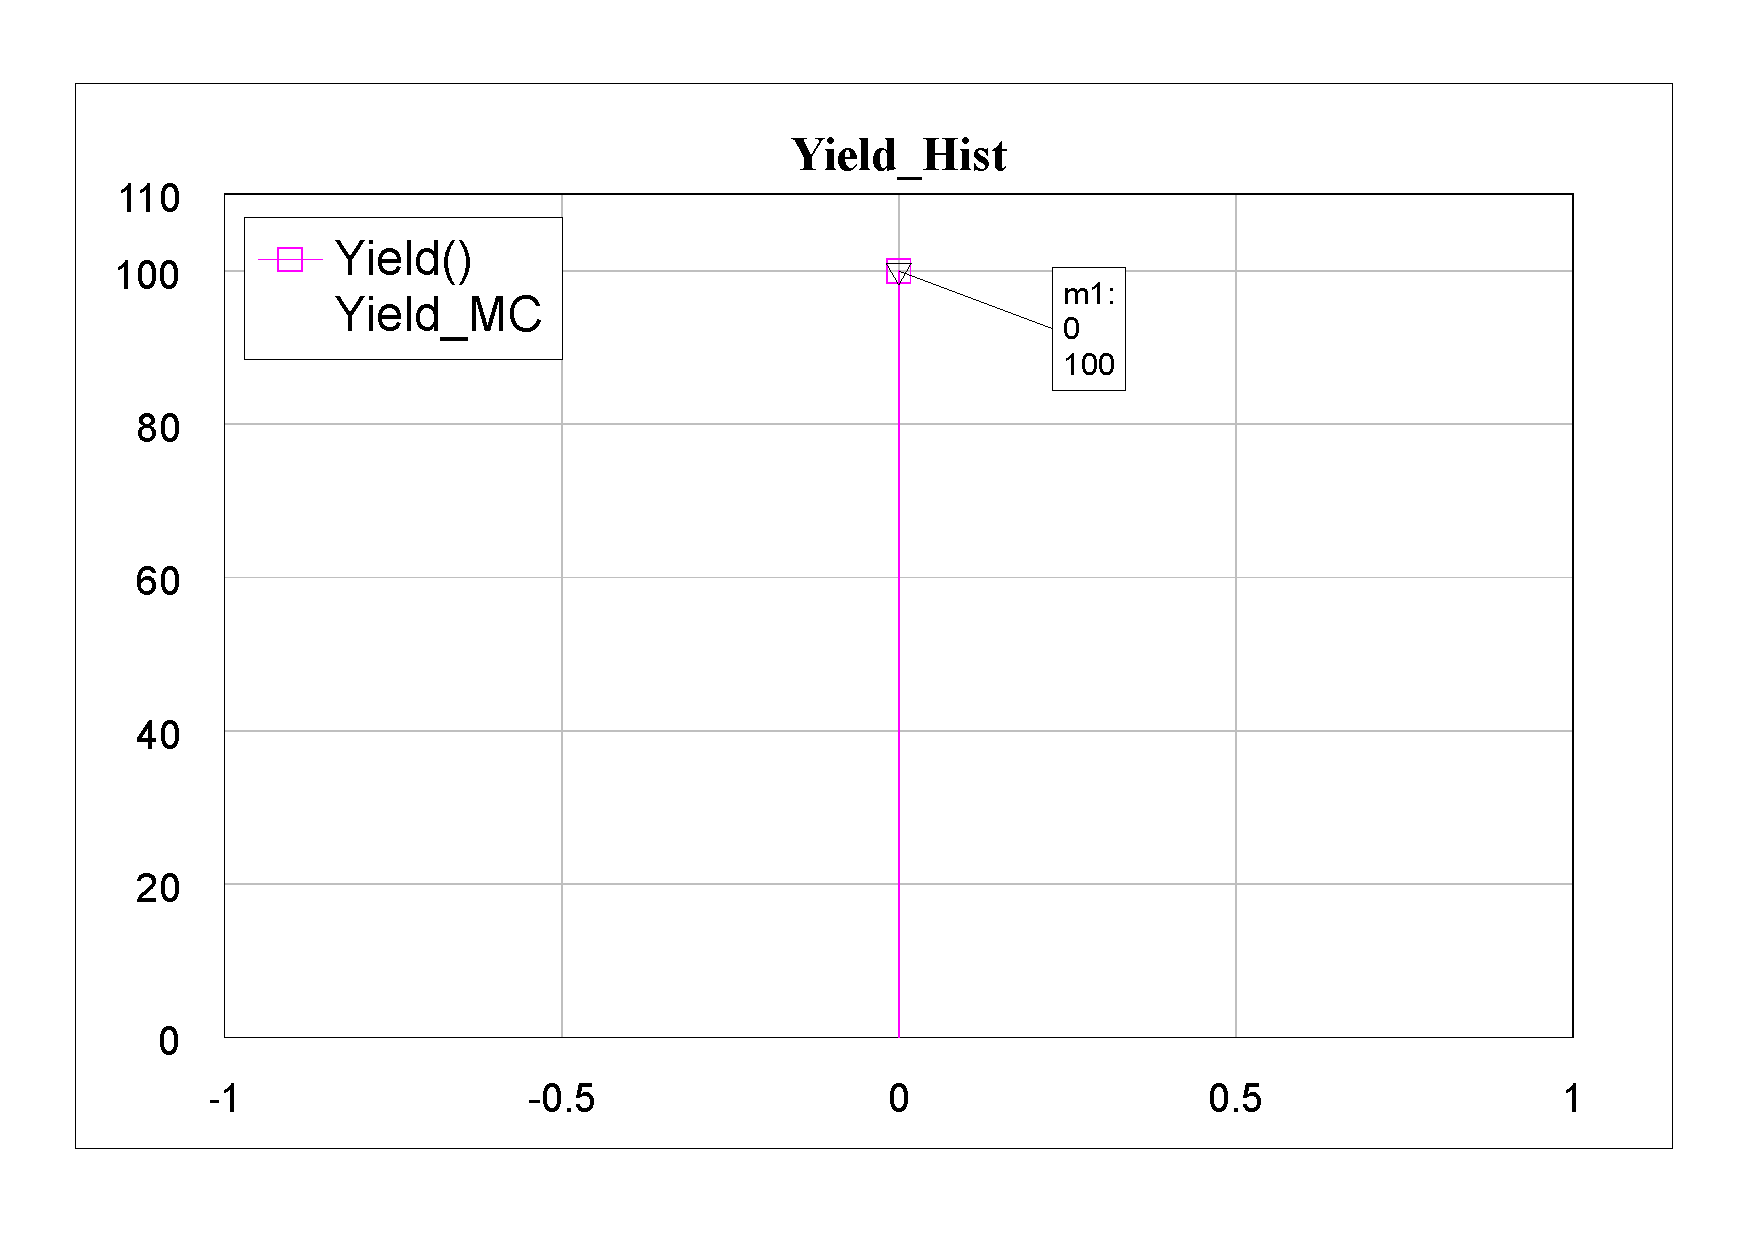
\includegraphics[width=\linewidth,height=5.8cm,keepaspectratio]{32_Yield.pdf}\\[2pt]
      {\scriptsize Kết quả Yield Analysis trên AWR (300 mẫu).}
    \end{column}
  \end{columns}
\end{frame}

% =====================================================================
\section{Kiểm chứng EM 3D (Ansys HFSS)}
% =====================================================================

% SLIDE 14
\begin{frame}{Mô phỏng EM 3D toàn sóng (Ansys HFSS, P2 $=30-j40\,\Omega$)}
  \centering
  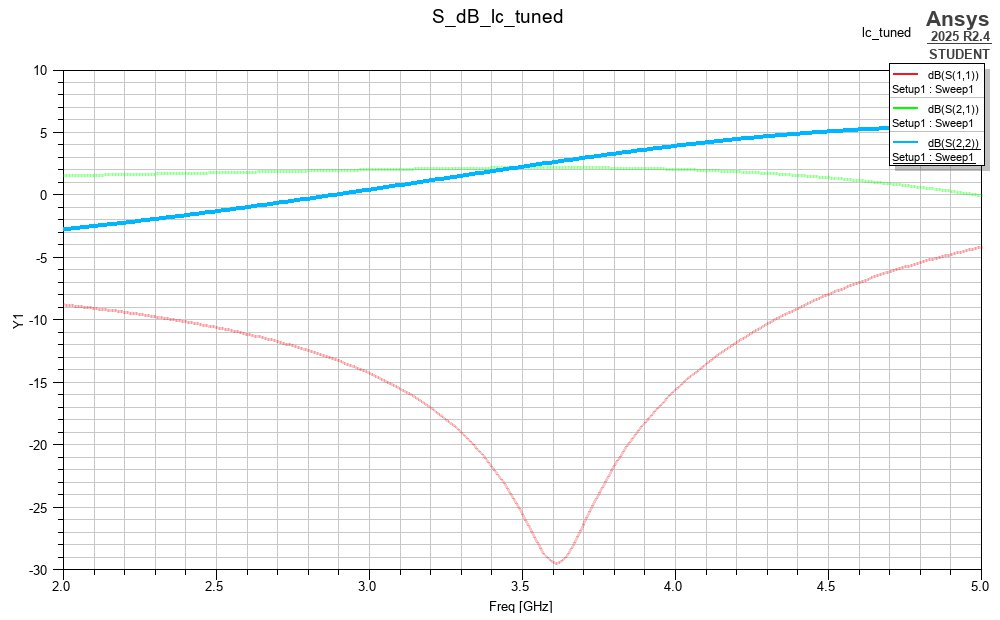
\includegraphics[width=0.32\linewidth,height=3.2cm,keepaspectratio]{33b_HFSS_lc_tuned.jpg}\hfill
  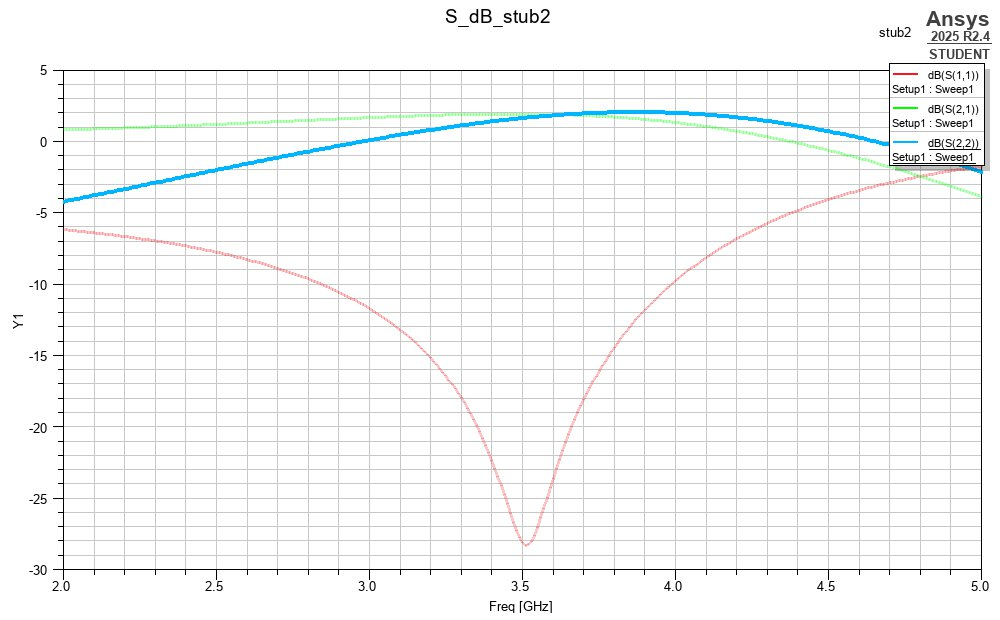
\includegraphics[width=0.32\linewidth,height=3.2cm,keepaspectratio]{33d_HFSS_stub2.jpg}\hfill
  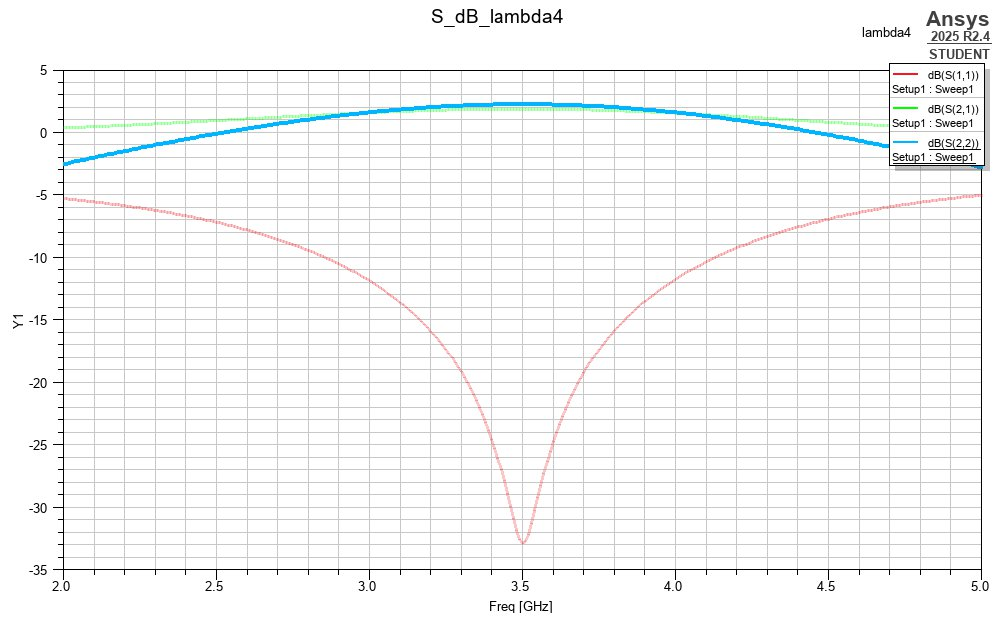
\includegraphics[width=0.32\linewidth,height=3.2cm,keepaspectratio]{33e_HFSS_lambda4.jpg}
  \vspace{2pt}
  \adjustbox{max width=\linewidth}{%
    \scriptsize
    \begin{tabular}{@{}lcccc@{}}
      \toprule
      \textbf{Cấu trúc (HFSS trên FR-4, P2 $=30-j40\,\Omega$)} & $f_{min}$ (GHz) & $S_{11}@3{,}5$ (dB) & $\mathrm{BW}_{-10\dB}$ & $G_T@3{,}5$ (dB) \\
      \midrule
      LC (chưa bù ký sinh via/pad) & $2{,}80$ & $-8{,}71$ & Không đạt & $-0{,}684$ \\
      \textbf{LC bù ký sinh} ($2{,}115\,$nH; $0{,}581\,$pF) & $3{,}61$ & $-25{,}55$ & $\mathbf{1950\MHz\,(55{,}7\%)}$ & $\mathbf{-0{,}041}$ \\
      Single-Stub (Nghiệm 2) & $3{,}51$ & $-28{,}10$ & $1130\MHz\,(32{,}3\%)$ & $-0{,}303$ \\
      \textbf{Biến áp $\lambda/4$ + dây đệm} & $\mathbf{3{,}50}$ & $\mathbf{-32{,}87}$ & $1260\MHz\,(36{,}0\%)$ & $-0{,}346$ \\
      \bottomrule
    \end{tabular}}
  \vspace{2pt}
  \begin{flushleft}
    {\scriptsize \textbf{Điểm nhấn:} Ký sinh via ($\approx0{,}78\,$nH) và pad kéo mạng LC lệch mạnh về $2{,}80\GHz$; sau bù ký sinh, cả 3 phương pháp khớp sát AWR và phủ trọn băng 5G n78 ($3{,}3$--$3{,}7\GHz$).}
  \end{flushleft}
\end{frame}

% =====================================================================
\section{So sánh tổng hợp \& Kết luận}
% =====================================================================

% SLIDE 15
\begin{frame}{Bảng so sánh tổng hợp 3 phương pháp theo 4 tiêu chí}
  \centering
  \adjustbox{max width=\linewidth}{%
    \renewcommand{\arraystretch}{1.35}
    \footnotesize
    \begin{tabular}{@{}p{2.6cm}p{4.0cm}p{4.0cm}p{4.0cm}@{}}
      \toprule
      \textbf{Tiêu chí} & \textbf{Mạng LC (L-section)} & \textbf{Single-Stub (Nghiệm 2)} & \textbf{Biến áp $\lambda/4$ + dây đệm} \\
      \midrule
      \textbf{Băng thông $-10\dB$} (AWR) & \textbf{Rộng nhất:} $2323\MHz$ ($66{,}4\%$) & Hẹp nhất: $780\MHz$ ($22{,}3\%$) & Khá rộng: $1242\MHz$ ($35{,}5\%$) \\
      \textbf{Kích thước / Diện tích} & \textbf{Nhỏ nhất} (2 linh kiện rời); cần bù ký sinh PCB & Gọn trong nhóm vi dải: dài $14{,}65\,$mm, đồng $\approx44{,}4\,\mathrm{mm}^2$ & Lớn nhất: dài $16{,}385\,$mm, rộng $6{,}947\,$mm, đồng $\approx91{,}2\,\mathrm{mm}^2$ \\
      \textbf{Suy hao chèn $S_{21}$} & $0\dB$ (lý tưởng); $-0{,}029\dB$ (HFSS) & \textbf{$-0{,}211\dB$} (thấp nhất nhóm vi dải FR-4) & $-0{,}261\dB$ (vi dải FR-4) \\
      \textbf{Độ nhạy sai số \& Yield} & Nhạy $L$ ($350\MHz@\pm10\%$); ít nhạy $C$ ($30\MHz$) & Nhạy $l$ ($-90/+83\MHz@\pm10\%$); ít nhạy $W$ & Nhạy $L_{50}, L_t, \varepsilon_r$ ($13$--$19\MHz/1\%$); \textbf{Yield 100\%} \\
      \bottomrule
    \end{tabular}}
  \vspace{6pt}
  {\footnotesize Cả ba phương pháp (LC sau bù ký sinh, Single-Stub N2, Biến áp $\lambda/4$) đều phủ trọn dải 5G n78 ($3{,}3$--$3{,}7\GHz$) với $S_{11}<-10\dB$ trên cả AWR và EM 3D HFSS.}
\end{frame}

% SLIDE 16
\begin{frame}{Kết luận \& Khuyến nghị ứng dụng 5G băng n78}
  \begin{columns}[T,onlytextwidth]
    \begin{column}{0.32\textwidth}
      \begin{block}{1. Mạng LC}
        \footnotesize
        \begin{itemize}
          \item Băng thông rộng nhất ($66{,}4\%$) và kích thước nhỏ gọn nhất.
          \item Phù hợp thiết bị di động giới hạn diện tích.
          \item \textbf{Lưu ý:} bắt buộc bù ký sinh via/pad ở dải GHz.
        \end{itemize}
      \end{block}
    \end{column}
    \begin{column}{0.32\textwidth}
      \begin{exampleblock}{2. Biến áp $\lambda/4$ (Khuyến nghị)}
        \footnotesize
        \begin{itemize}
          \item Hoàn toàn vi dải, không cần linh kiện rời.
          \item Băng thông rộng ($35{,}5\%$), chịu dung sai xuất sắc (\textbf{Yield 100\%}).
          \item \textbf{Lưu ý:} rút ngắn $L_t \approx 7\%$ khi tinh chỉnh PCB.
        \end{itemize}
      \end{exampleblock}
    \end{column}
    \begin{column}{0.32\textwidth}
      \begin{block}{3. Single-Stub (Nghiệm 2)}
        \footnotesize
        \begin{itemize}
          \item Vi dải gọn hơn $\lambda/4$ ($\approx44{,}4\,\mathrm{mm}^2$), suy hao thấp nhất nhóm vi dải ($0{,}211\dB$).
          \item Băng thông hẹp hơn ($22{,}3\%$) và nhạy chiều dài stub $l$.
        \end{itemize}
      \end{block}
    \end{column}
  \end{columns}
  \vspace{6pt}
  \begin{alertblock}{Hướng phát triển}
    \small
    Chế tạo mạch thực tế trên nền PCB FR-4 ($\varepsilon_r=4{,}4$, $h=1{,}6\,$mm) và đo kiểm nghiệm tham số tán xạ ($S_{11}$, $S_{21}$) bằng máy phân tích mạng vector (VNA).
  \end{alertblock}
\end{frame}

% =====================================================================
% SLIDE 17: CẢM ƠN
% =====================================================================
\begin{frame}[plain]
  \vfill
  \begin{center}
    {\usebeamerfont{title}\usebeamercolor[fg]{title}\Huge\bfseries Cảm ơn Thầy và các bạn đã lắng nghe!}\\[14pt]
    {\large Rất mong nhận được câu hỏi và góp ý.}\\[18pt]
    {\small\color{gray} Tổ 8 -- Nhóm L04 \quad\textbar\quad Kỹ thuật Siêu cao tần \quad\textbar\quad GVHD: TS. Nguyễn Minh Tân}
  \end{center}
  \vfill
\end{frame}

\end{document}
